\def\year{2021}\relax
%File: formatting-instructions-latex-2021.tex
%release 2021.2
\documentclass[letterpaper]{article} % DO NOT CHANGE THIS
\usepackage{aaai21}  % DO NOT CHANGE THIS
\usepackage{times}  % DO NOT CHANGE THIS
\usepackage{helvet} % DO NOT CHANGE THIS
\usepackage{courier}  % DO NOT CHANGE THIS
\usepackage[hyphens]{url}  % DO NOT CHANGE THIS
\usepackage{graphicx} % DO NOT CHANGE THIS
\urlstyle{rm} % DO NOT CHANGE THIS
\def\UrlFont{\rm}  % DO NOT CHANGE THIS
\usepackage{natbib}  % DO NOT CHANGE THIS AND DO NOT ADD ANY OPTIONS TO IT
\usepackage{caption} % DO NOT CHANGE THIS AND DO NOT ADD ANY OPTIONS TO IT
\frenchspacing  % DO NOT CHANGE THIS
\setlength{\pdfpagewidth}{8.5in}  % DO NOT CHANGE THIS
\setlength{\pdfpageheight}{11in}  % DO NOT CHANGE THIS

\usepackage{booktabs}
\usepackage{amsmath}
\usepackage{algorithmic}
\usepackage{textcomp}
\usepackage{xcolor}
\usepackage{fancyhdr}
\usepackage{float}

%\nocopyright
%PDF Info Is REQUIRED.
% For /Author, add all authors within the parentheses, separated by commas. No accents or commands.
% For /Title, add Title in Mixed Case. No accents or commands. Retain the parentheses.
\pdfinfo{
/Title (Conference Submission)
/Author (Feng Shi, Chonghan Lee, Liang Qiu, Yizhou Zhao, Tianyi Shen, Shivran Muralidhar, Tian Han, Song-Chun Zhu, Vijaykrishnan Narayanan)
/TemplateVersion (2021.2)
} %Leave this
% /Title ()
% Put your actual complete title (no codes, scripts, shortcuts, or LaTeX commands) within the parentheses in mixed case
% Leave the space between \Title and the beginning parenthesis alone
% /Author ()
% Put your actual complete list of authors (no codes, scripts, shortcuts, or LaTeX commands) within the parentheses in mixed case.
% Each author should be only by a comma. If the name contains accents, remove them. If there are any LaTeX commands,
% remove them.

% DISALLOWED PACKAGES
% \usepackage{authblk} -- This package is specifically forbidden
% \usepackage{balance} -- This package is specifically forbidden
% \usepackage{color (if used in text)
% \usepackage{CJK} -- This package is specifically forbidden
% \usepackage{float} -- This package is specifically forbidden
% \usepackage{flushend} -- This package is specifically forbidden
% \usepackage{fontenc} -- This package is specifically forbidden
% \usepackage{fullpage} -- This package is specifically forbidden
% \usepackage{geometry} -- This package is specifically forbidden
% \usepackage{grffile} -- This package is specifically forbidden
% \usepackage{hyperref} -- This package is specifically forbidden
% \usepackage{navigator} -- This package is specifically forbidden
% (or any other package that embeds links such as navigator or hyperref)
% \indentfirst} -- This package is specifically forbidden
% \layout} -- This package is specifically forbidden
% \multicol} -- This package is specifically forbidden
% \nameref} -- This package is specifically forbidden
% \usepackage{savetrees} -- This package is specifically forbidden
% \usepackage{setspace} -- This package is specifically forbidden
% \usepackage{stfloats} -- This package is specifically forbidden
% \usepackage{tabu} -- This package is specifically forbidden
% \usepackage{titlesec} -- This package is specifically forbidden
% \usepackage{tocbibind} -- This package is specifically forbidden
% \usepackage{ulem} -- This package is specifically forbidden
% \usepackage{wrapfig} -- This package is specifically forbidden
% DISALLOWED COMMANDS
% \nocopyright -- Your paper will not be published if you use this command
% \addtolength -- This command may not be used
% \balance -- This command may not be used
% \baselinestretch -- Your paper will not be published if you use this command
% \clearpage -- No page breaks of any kind may be used for the final version of your paper
% \columnsep -- This command may not be used
% \newpage -- No page breaks of any kind may be used for the final version of your paper
% \pagebreak -- No page breaks of any kind may be used for the final version of your paperr
% \pagestyle -- This command may not be used
% \tiny -- This is not an acceptable font size.
% \vspace{- -- No negative value may be used in proximity of a caption, figure, table, section, subsection, subsubsection, or reference
% \vskip{- -- No negative value may be used to alter spacing above or below a caption, figure, table, section, subsection, subsubsection, or reference

\setcounter{secnumdepth}{0} %May be changed to 1 or 2 if section numbers are desired.

% The file aaai21.sty is the style file for AAAI Press
% proceedings, working notes, and technical reports.
%

% Title

% Your title must be in mixed case, not sentence case.
% That means all verbs (including short verbs like be, is, using,and go),
% nouns, adverbs, adjectives should be capitalized, including both words in hyphenated terms, while
% articles, conjunctions, and prepositions are lower case unless they
% directly follow a colon or long dash

\title{STAR: \underline{S}parse \underline{T}ransformer-based \underline{A}ction \underline{R}ecognition}
\author{
    %Authors
    % All authors must be in the same font size and format.
    
    % Written by AAAI Press Staff\textsuperscript{\rm 1}\thanks{With help from the AAAI Publications Committee.}\\
    % AAAI Style Contributions by Pater Patel Schneider,
    % Sunil Issar,  \\
    % J. Scott Penberthy,
    % George Ferguson,
    % Hans Guesgen,
    % Francisco Cruz,
    % Marc Pujol-Gonzalez
    % \\
    
    Feng Shi\textsuperscript{\rm 1}, 
    Chonghan Lee\textsuperscript{\rm 2}, 
    Liang Qiu\textsuperscript{\rm 1}, 
    Yizhou Zhao\textsuperscript{\rm 1}, 
    Tianyi Shen\textsuperscript{\rm 2}, 
    Shivran Muralidhar\textsuperscript{\rm 2}, 
    Tian Han\textsuperscript{\rm 3},
    Song-Chun Zhu\textsuperscript{\rm 1}, 
    Vijaykrishnan Narayanan\textsuperscript{\rm 2}
    \\
}
\affiliations{
    %Afiliations
    \textsuperscript{\rm 1}University of California Los Angeles\\
    %If you have multiple authors and multiple affiliations
    % use superscripts in text and roman font to identify them.
    %For example,

    % Sunil Issar, \textsuperscript{\rm 2}
    % J. Scott Penberthy, \textsuperscript{\rm 3}
    % George Ferguson,\textsuperscript{\rm 4}
    % Hans Guesgen, \textsuperscript{\rm 5}.
    % Note that the comma should be placed BEFORE the superscript for optimum readability

    \textsuperscript{\rm 2}The Pennsylvania State University\\
    % email address must be in roman text type, not monospace or sans serif
    \textsuperscript{\rm 3}Stevens Institute of Technology\\

    % See more examples next
}
\iffalse
%Example, Single Author, ->> remove \iffalse,\fi and place them surrounding AAAI title to use it
\title{My Publication Title --- Single Author}
\author {
    % Author
    Author Name \\
}

\affiliations{
    Affiliation \\
    Affiliation Line 2 \\
    name@example.com
}
\fi

\iffalse
%Example, Multiple Authors, ->> remove \iffalse,\fi and place them surrounding AAAI title to use it
\title{My Publication Title --- Multiple Authors}
\author {
    % Authors
    First Author Name,\textsuperscript{\rm 1}
    Second Author Name, \textsuperscript{\rm 2}
    Third Author Name \textsuperscript{\rm 1} \\
}
\affiliations {
    % Affiliations
    \textsuperscript{\rm 1} Affiliation 1 \\
    \textsuperscript{\rm 2} Affiliation 2 \\
    firstAuthor@affiliation1.com, secondAuthor@affilation2.com, thirdAuthor@affiliation1.com
}
\fi
\begin{document}

\maketitle

\begin{abstract}
The cognitive system for human action and behavior has evolved into a deep learning regime, and especially the advent of Graph Convolution Networks has transformed the field in recent years. However, previous works have mainly focused on over-parameterized and complex models based on dense graph convolution networks, resulting in low efficiency in training and inference. Meanwhile, the Transformer architecture-based model has not yet been well explored for cognitive application in human action and behavior estimation. This work proposes a novel skeleton-based human action recognition model with sparse-attention on the spatial dimension and segmented linear attention on the temporal dimension of data. Our model can also process variable length of video clips grouped as a single batch. Experiments show that our model can achieve comparable performance while utilizing much less trainable parameters and achieve high speed in training and inference. Experiments show that our model achieves 4$\sim$18$\times$ speedup and $\frac{1}{7}$$\sim$$\frac{1}{15}$ model size compared with the baseline models at competitive accuracy.
\end{abstract}

\section{Introduction}
Human action recognition plays a crucial role in many real-world applications, such as holistic scene understanding, video surveillance, and human-computer interaction \cite{vsurveilance, hcinter/978-3-540-78566-8_10}. In particular, skeleton-based human action recognition has attracted much attention in recent years and has shown its effectiveness. The skeleton representation contains a time series of 2D or 3D coordinates of human key-joints, providing dynamic body movement information that is robust to variations of light conditions and background noises in contrast to raw RGB representation.

Earlier skeleton-based human action recognition methods focus on designing hand-crafted features extracted from the joint coordinates \cite{lie2014, actionlet2012} and aggregating learned features using RNNs and CNNs \cite{rnndu, xiememory, zhang2017view, ts3dliu, tdskrepke}. However, these methods rarely explore the relations between body joints and result in unsatisfactory performance. Recent methods focus on exploring the natural connection of human body joints and successfully adopted the Graph Convolutional Networks (GCNs), especially for non-Euclidean domain data, similar to Convolutional Neural Networks (CNNs) but executing convolutional operations to aggregate the connected and related joints' features. Yan et al. \cite{yan2018spatial} proposed a ST-GCN model to extract discriminative features from spatial and temporal graphs of body joints. Following the success of ST-GCN, many works proposed optimizations to ST-GCN to improve the performance and network capacity \cite{directed2019, Li_2019_CVPR, liu2020disentangling}.

However, the existing GCN-based models are often impractical in real-time applications due to their vast computational complexity and memory usage. The baseline GCN model, e.g., ST-GCN, consists of more than 3.09 million parameters and costs at least 16.2 GFLOPs to run inference on a single action video sample \cite{yan2018spatial}. DGNN, which is composed of incremental GCN modules, even contains 26 million model parameters. \cite{directed2019} Such high model complexity leads to difficulty in model training and inference, makes the model not suitable for deployment on edge devices. Furthermore, these GCN-based models process fixed-size action videos by padding repetitive frames and zeros to match the maximum number of frames and persons depicted in the videos. These additional paddings increase the latency and memory required hindering their adoption in real-time and embedded applications.

This paper proposes a \textit{sparse transformer-based action recognition} (STAR) model as a novel baseline for skeleton action modeling to address the above shortcomings. Transformers have been a popular choice in natural language processing. Recently, they have been employed in computer vision to attain competitive results compared to convolutional networks, while requiring fewer computational resources to train \cite{dosovitskiy2020image, huang2019ccnet}. Inspired by these Transformer architectures, our model consists of spatial and temporal encoders, which apply sparse attention and segmented linear attention on skeleton sequences along the spatial and temporal dimension, respectively.
% GCN are not necessarily to be dense, ST-GCN alike models are adopting dense version, (we don't know why they are using such kind of design, hehe)
Our sparse attention module along the spatial dimension performs sparse matrix multiplications to extract correlations of connected joints, whereas previous approaches utilize dense matrix multiplications where most of the entries are zeros, causing extra computation. The segmented linear attention mechanism along temporal dimension further reduces the computation and memory usage by processing variable length of sequences. We also apply segmented positional encoding to the data embedding to provide the concept of time-series ordering along the temporal dimension of variable-length skeleton data. Additionally, segmented context attention performs weighted summarization across the entire video frames, making our model robust compared to GCN-based models with their fixed-length receptive field on the temporal dimension.

Compared to the baseline GCN model (ST-GCN), our model (STAR) achieves higher performance with much smaller model size on the two datasets, NTU RGB+D 60 and 120. The major contributions of this work are listed below:
\begin{itemize}
    \item We focus on designing an efficient model purely based on self-attention mechanism. We propose \textit{sparse transformer-based action recognition} (STAR) model that process variable length of skeleton action sequence without additional preprocessing and zero paddings. The flexibility of our model is beneficial for real-time applications or edge platforms with limited computational resources.
    \item  We propose a sparse self-attention module that efficiently performs sparse matrix multiplications to capture spatial correlations between human skeleton joints.
    \item We propose a segmented linear self-attention module that effectively captures temporal correlations of dynamic joint movements across time dimension.
    \item Experiments show that our model is 5$\sim$7$\times$ smaller than the baseline models while providing 4$\sim$18$\times$ execution speedup.
\end{itemize}

\section{Related works}
\subsection{Skeleton-Based Action Recognition}
Recently, skeleton-based action recognition has attracted much attention since its compact skeleton data representation makes the models more efficient and free from the variations in lighting conditions and other environmental noises. Earlier methods to skeleton-based action modeling have mainly worked on designing hand-crafted features and relations between joints \cite{}. %TODO: citation
Recently, by looking into the inherent connectivity of the human body, Graph Convolutional Networks (GCNs), especially, ST-GCNs have gained massive success in getting satisfactory results in this task. The model consists of spatial and temporal convolution modules similar to conventional convolutional filters used for images \cite{yan2018spatial}. The graph adjacency matrix encodes the skeleton joints' connections and extracts high-level spatial representations from the skeleton action sequence. On the temporal dimension, 1D convolutional filters facilitate extracting dynamic information.

Many following works have proposed improvements to ST-GCN to improve the performance. Li et al. \cite{Li_2019_CVPR} proposed AS-GCN, which leveraged the potential of adjacency matrices to scale the human skeleton's connectivity. Furthermore, they generated semantic links to capture better structural and action semantics with additional information aggregation. Lei et al. \cite{shi2019skeleton} proposed Directed Graph Neural Networks (DGNNs), which incorporate joint and bone information to represent the skeleton data as a directed acyclic graph. Liu et al. \cite{liu2020disentangling} proposed a unified spatial-temporal graph convolution module (G3D) to aggregate information across space and time for effective feature learning.

Some studies have been focusing on the computational complexity of GCN-based methods. Cheng et al. \cite{cheng2020shiftgcn} proposed Shift-GCN, which leverages shift graph operations and point-wise convolutions to reduce the computational complexity. Song et al. \cite{song2020stronger} proposed multi-branch ResGCN that fuses different spatio-temporal features from multiple branches and used residual bottleneck modules to obtain competitive performance with less number of parameters. Compared to these methods, our spatial and temporal self-attention modules have several essential distinctions: our model can process variable length of skeleton sequence without preprocessing with zero-paddings. Our model can retrieve global context on the temporal dimension by applying self-attention to the input sequence's entire frames.

\subsection{Transformers and Self-Attention Mechanism}
Vaswani et al. \cite{attn2017all} first introduced Transformers for machine translation and have been the state-of-the-art method in various NLP tasks. For example, GPT and BERT \cite{radford2018improving, devlin-etal-2019-bert} are currently the Transformer-based language models that have achieved the best performance. The core component of Transformer architectures is a self-attention mechanism that learns the relationships between each element of a sequence. In contrast to recurrent networks that process sequence in a recursive fashion and are limited to attention on short-term context, transformer architectures enable modeling long dependencies in sequence. Furthermore, the multi-head self-attention operations can be easily parallelized. Recently, Transformer-based models have attracted much attention in the computer vision community. Convolution operation has been the core of the conventional deep learning models for computer vision tasks. However, there are downfalls to the operation. The convolution operates on a fixed-sized window, which only captures short-range dependencies. The same applies to GCNs where the Graph Convolution operation is incapable of capturing long-range relations between joints in both spatial and temporal dimensions. 

Vision Transformer (ViT) \cite{dosovitskiy2020image} is the first work to completely replace standard convolutions in deep neural networks on large-scale image recognition tasks. Huang et al. \cite{huang2019ccnet} explored the sparse attention to study the trade-off between computational efficiency and performance of a Transformer model on the image classification task. A recent study \cite{plizzari2020spatial} proposed a hybrid model consists of the Transformer encoder and GCN modules on the skeleton-based human action recognition task. Nevertheless, no prior study has completely replaced GCNs with the Transformer architecture to the best of our knowledge.

% ---------------------- Methodology -------------------------
\section{Methodology}
 
In this section, we present the algorithms used in our model and the relevant architecture of our model. 

Section \ref{sec:sparse_attn} depicts the \textbf{sparse multi-head self-attention} (MHSA) mechanism used in spatial Transformer encoder module; Section \ref{sec:temp_attn} introduces the novel data format and the relevant \textbf{linear multi-head self-attention} (MHSA) mechanism for temporal Transformer encoder; Section \ref{sec:arch} shows the overall framework of our model and related auxiliary modules.

\begin{figure}[ht]
    \centering
    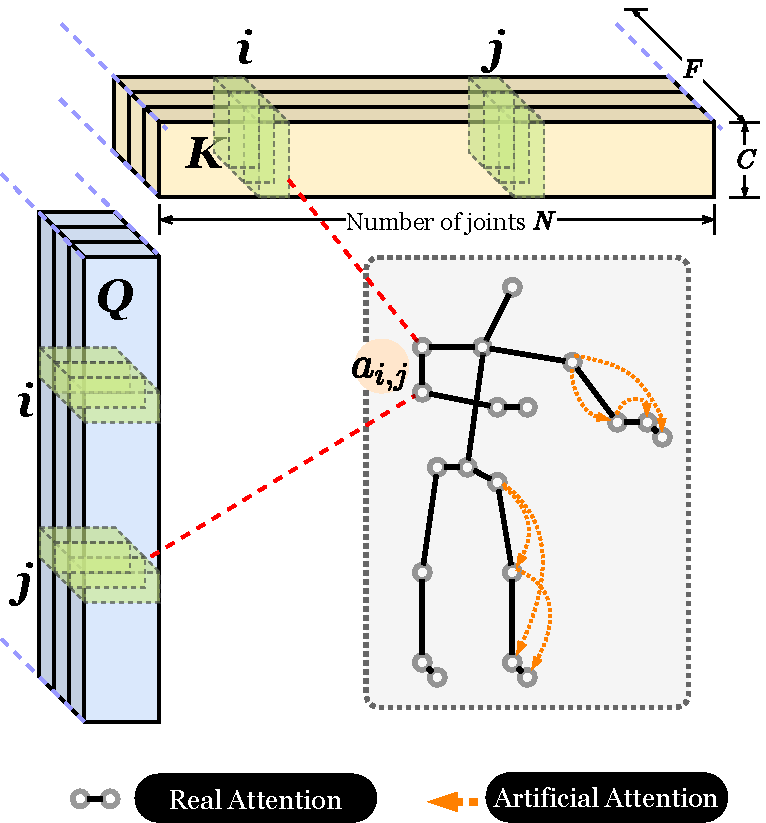
\includegraphics[width=0.3\textwidth]{sparse_attn2.pdf}
    \caption{Illustration of our Sparse attention module: Given the queries $Q$ and the keys $K$ of the skeleton embedding, feature vectors of joint $i$ and $j$ are correlated with attention weight $\alpha_{i,j}$ The solid black line on the skeleton represents the physical connection of human skeleton. The dashed line connecting two joints represents the artificial attention of joints.}
    \label{fig:sparse_attn}
\end{figure}

\subsection{Spatial domain: Sparse MHSA} \label{sec:sparse_attn}

The crucial component of our \textit{spatial transformer encoder} is the \textit{sparse multi-head self-attention} module. GCN-based models and previous Transformer models, such as ST-GCN and ST-TR, utilize dense skeleton representation to aggregate the features of neighboring nodes. This dense adjacency matrix representation contains 625 entries for the NTU dataset, while the actual number of joint connections representing the skeletons is only 24. It means that 96\% of the matrix multiplications are unnecessary calculations for zero entries. So we propose a sparse attention mechanism, which only performs matrix multiplications on the sparse node connections. This allows each joint to only aggregate the information from its neighboring joints based on the attention coefficients, which are dynamically assigned to the corresponding connections.

The joint connections are based on the topology of skeleton, which is a tree structure. The attentions inherited from this topology are seen as \textit{physical attention} (or \textit{real attention}), as illustrated in Figure \ref{fig:sparse_attn}. To augment the attending field, we also artificially add more links between joints according to the logical relations of body parts, and we call these artificially created attentions as \textit{artificial attention}, as the dashed yellow arrows shown in Figure \ref{fig:sparse_attn}. For simplicity, suppose that the skeleton adjacency matrix is $A$, then the artificial links for additional spatial attention are obtained through $A^2$ and $A^3$. Hence, in our model, the spatial attention maps are evaluated based on the topology representation of $A + A^2 + A^3$.

The sparse attention is calculated according to the connectivity between joints. As described in below equations: after the embedding in Equation \ref{eq:embedding}, the joint-to-joint attention between a pair of connected joints is computed first by an exponential score of the dot product of the feature vectors of these two joints (Equation \ref{eq:attn}), then the score is normalized by the sum of exponential scores of all neighboring joints as described in Equation \ref{eq:sparse_attn}.
\begin{align}
    Q &= X W_q, K = X W_k, V = X W_v \label{eq:embedding}\\
    \alpha_{i, j} &= \frac{\left<q_i, k_j\right>}{\sum_{n \in N(i)} \left< q_i, k_n \right>}
   \label{eq:attn} \\
    v_{i}' &= \sum_{j \in N(i)} \alpha_{i, j} v_j, \quad\text{ or }  V' = \mathcal{A} V
    \label{eq:sparse_attn}
\end{align}

where $Q$, $K$, and $V$ are queries, keys, and values in Transformer's terminology, respectively; and $q_i = Q(i)$, $k_j = K(j)$, $v_j = V(j)$, and $\left< q, k \right> = exp\left( \frac{q^T k}{\sqrt{d}} \right)$. Finally, we obtain attention maps $\mathcal{A}$ as multi-dimension (multi-head) sparse matrices sharing the identical topology described by a single adjacency matrix (including links for the artificial attention), where attention coefficients are $\mathcal{A}(i, j) = \alpha_{i, j}$. The sparse operation can be fulfilled with tensor gathering and scattering operations for parallelism.

\subsection{Temporal domain: Segmented Linear MHSA} \label{sec:temp_attn}
\begin{figure}[ht]
    \centering
    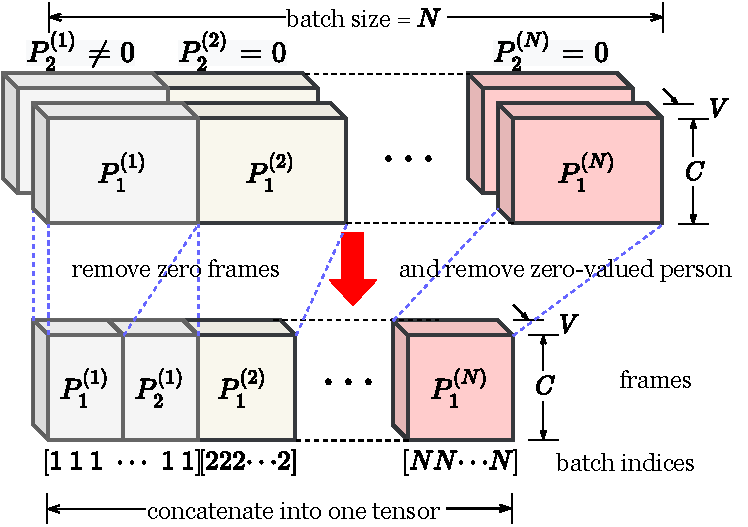
\includegraphics[width=0.4\textwidth]{data_format.pdf}
    \caption{Illustration of our data format used in our framework: Previous works used the upper data format, which has fixed-sized time and person dimensions. Our work adopts new data format on the bottom, which has combined batch, person, and time dimensions into a single  variable length sequence.}
    \label{fig:data_format}
\end{figure}

The most apparent drawbacks in the previous approaches \cite{yan2018spatial, 2sagcn2019cvpr} are utilizing (1) the fixed number of frames for each video clip and (2) zero-filling for the non-existing second person. The first drawback constrains their scalability to process video clips longer than the predefined length and their flexibility on a shorter video clip. The second drawback due to the zero's participation in computation causes latency degradation. Moreover, a significant amount of memory space is allocated to those zero-valued data during the computation. So we propose a compact data format to bypass these drawbacks. Also, we propose Segmented Linear MHSA to process our compact data format.

\begin{figure*}[ht]
    \centering
    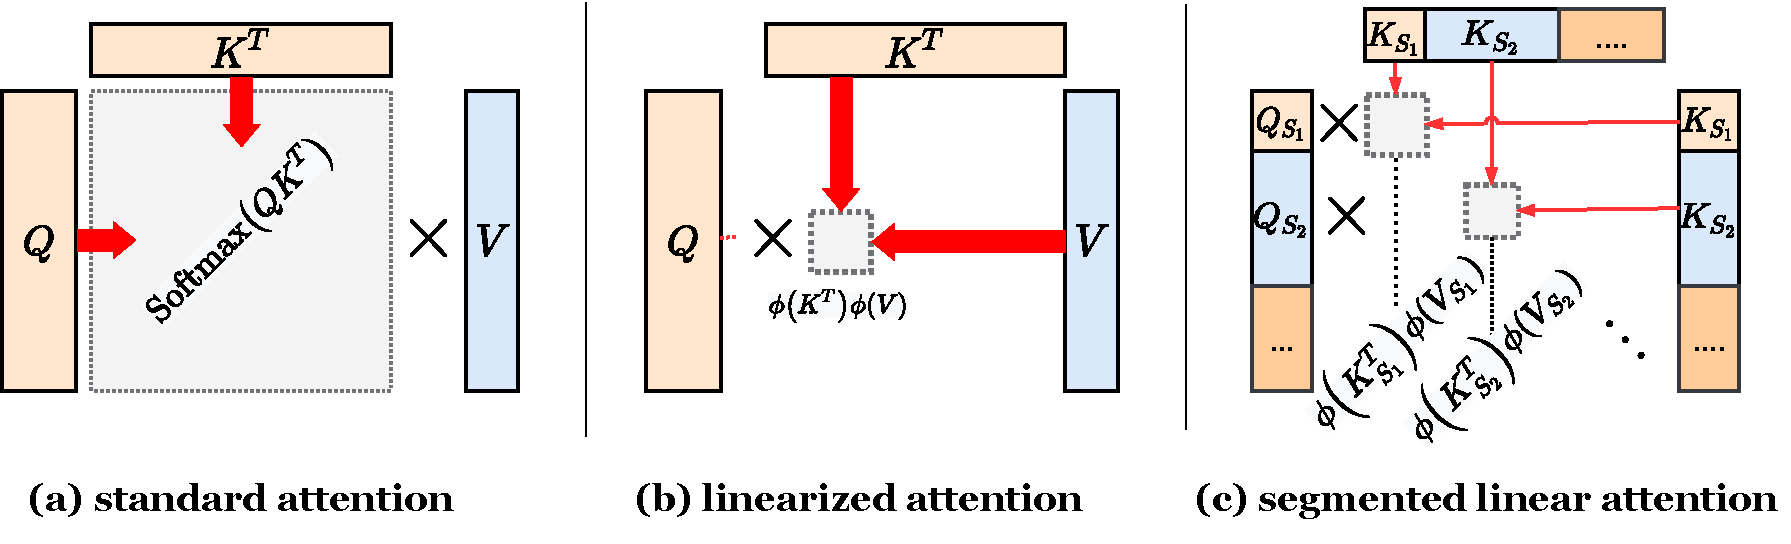
\includegraphics[width=0.8\textwidth]{attn_ops.pdf}
    \caption{Illustration of Different Attention Operations: (a) Standard attention is obtained from $Softmax(QK^T)V$ with a complexity of $\mathcal{O}(n^2)$. (b) Linearized attention $\phi(Q) (\phi(K^T) V)$ with kernel function $\phi(\cdot)$ reduces the complexity to $\mathcal{O}(n)$, (c) we extend the linearized attention (b) to process segments of sequences.}
    \label{fig:attn_ops}
\end{figure*}

\subsubsection{Variable Frame Length Data Format} 
The Figure \ref{fig:data_format} shows the comparison between our data format and the format used by previous works. In the data format adopted by previous works, longer videos are cut off to the predefined length and shorter videos are padded with repeated frames. Furthermore, the frames with a single person are all zero-padded to match the fixed number of persons. The upper data format from Figure\ref{fig:data_format} illustrates the NTU RGB+D data format used by previous works. In each fixed-length video $V^{(i)}$, $P_1^{(i)}$ and $P_2^{(i)}$ represent two persons. In NTU RGB+D 120 dataset, only 26 out of 120 actions are mutual actions, which means that the second person's skeleton is just zeros ($P_2^{(i)} = 0$ in Figure \ref{fig:data_format}) in most data samples. In contrast to the previous data format, the proposed format maintains the original length of each video clip. Additionally, when a video clip contains two persons, we concatenate them along the frame dimension. Instead of keeping an individual dimension for a batch of video clips, we further concatenate the video clips in a batch along the frame dimension, and the auxiliary vector stores the batch indices to indicate to which video clip a frame belongs, as shown in the bottom data format of Figure \ref{fig:data_format}. Moreover, given the new dimensions ($N$, $V$, $C$) as shown in Figure \ref{fig:data_format}, where $N$ is the total number of frames after concatenating the video clips along the temporal dimension and $V$ is the number of skeleton's joints, we regard dimension $N$ as the logical batch size for spatial attention and dimension $V$ as the logical batch size for temporal attention.

\begin{figure}[ht]
    \centering
    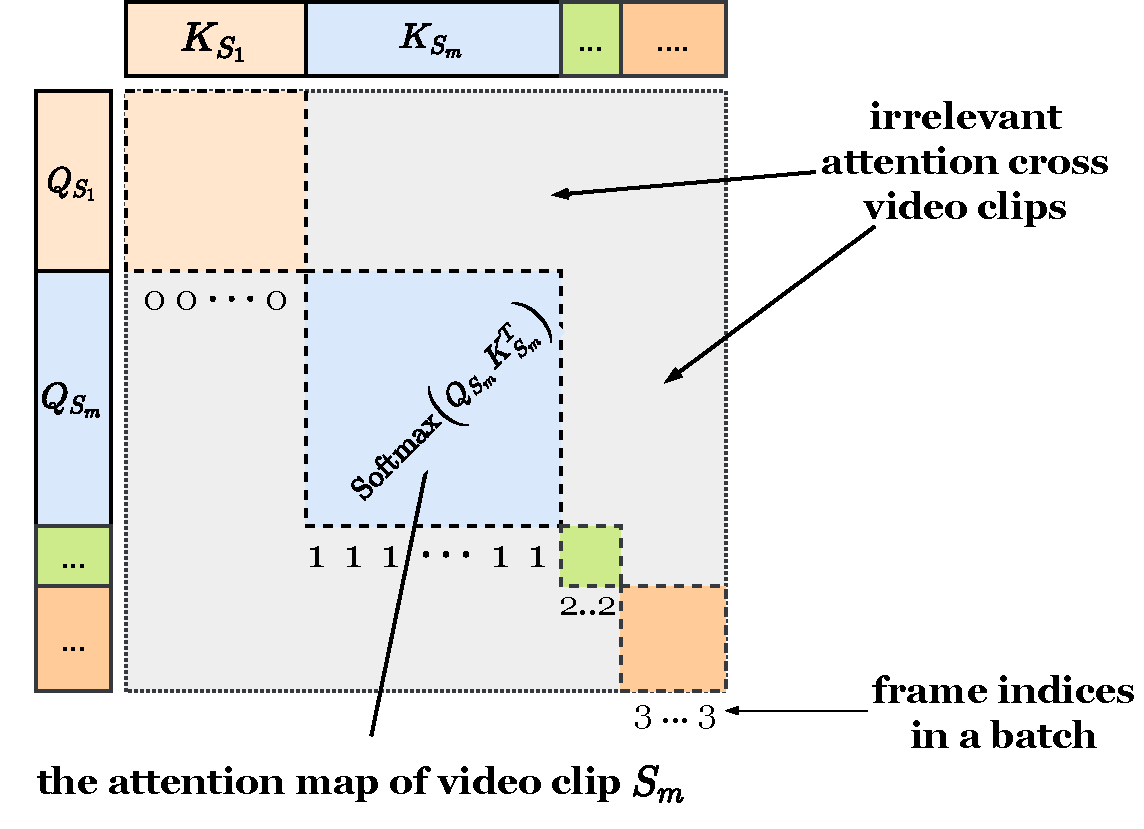
\includegraphics[width=0.45\textwidth]{sgm_attn.pdf}
    \caption{Segmented Attention: directly applying the linearized attention to our new data format will calculate unexpected attention between the two irrelevant video clips, which is error-prone. Therefore, we use segmented attention corresponding to each video sequence.}
    \label{fig:sgm_attn}
\end{figure}

\subsubsection{Segmented Linear Attention} \label{linear_attn}
With the new data format introduced in the previous section, we propose a novel linear multi-head attention tailored for this data format. We call it a Segmented Linear Attention. As stated in the previous sections, Transformers are originally designed for sequential data. In the human skeleton sequence, each joint's dynamic movement across the frames can be regarded as a time series. Therefore, the 3D coordinates, i.e., $(x, y, z)$, of every joint can be processed individually through the trajectory along the time dimension, and the application of attention extracts the interaction among time steps represented by frames. 

\textbf{Linear Attention}. Standard dot product attention mechanism \cite{attn2017all} (Equation \ref{eq:std_attn}) with the global receptive field of $N$ inputs are prohibitively slow due to the quadratic time and memory complexity $\mathcal{O}(N^2)$. The quadratic complexity also makes Transformers hard to train and limits the context. Recent research toward the linearized attention mechanism derives the approximation of the \textit{Softmax}-based attention. The most appealing ones are linear Transformers \cite{katharopoulos20a, choromanski2021rethinking, shen2021efficient} based on kernel functions approximating the \textit{Softmax}. The linearized Transformers can improve inference speeds up to three orders of magnitude without much loss in predictive performance \cite{tay2020efficient}.
Given the projected embeddings $Q$, $K$, and $V$ for input tensors of queries, keys, and values, respectively, according to the observation from the accumulated value $V_i' \in \mathbf{R}^{d}$ for the query $Q_i \in \mathbf{R}^{d}$ in position $i$, $d$ is the channel dimension, the linearized attention can be transformed from Equation \ref{eq:std_attn} to Equation \ref{eq:lnr_attn}, the computational complexity is reduced to $\mathcal{O}(Nd)$, when $d$ is much smaller than $N$, the computational complexity is approaching linear $\mathcal{O}(N)$:
\begin{equation}
    V_i' = \frac{\sum_{j=1}^N \left< Q_i, K_j \right> V_j}{\sum_{j=1}^N \left< Q_i, K_i \right>}
    \label{eq:std_attn}
\end{equation}

\begin{equation}
    \begin{split}
        V_i' &= \frac{\phi(Q_i)^T \sum_{j=1}^N \phi(K_j) V_j^T}{\phi(Q_i)^T \sum_{j=1}^N \phi(K_j)} = \frac{\phi(Q_i)^T U}{\phi(Q_i)^T Z} \\ 
        U &= \sum_{j=1}^N \phi(K_j) V_j^T, \quad Z = \sum_{j=1}^N \phi(K_j)
    \end{split}
    \label{eq:lnr_attn}
\end{equation}

where $\phi(\cdot)$ is the kernel function. In work of \cite{katharopoulos20a}, kernel function is simply simulated with ELU, $\phi(x) = elu(x) + 1$; while \cite{choromanski2021rethinking} introduces the \textit{Fast Attention via Orthogonal Random Feature} (FAVOR) maps as the kernel function, $\phi(x) = \frac{c}{\sqrt{M}} f(W x + b)^T$, where $c > 0$ is a constant, and $W \in \mathbf{R}^{M \times d}$ is a Gaussian random feature matrix, and $M$ is the dimensionality of this matrix that controls the number of random features.

\begin{figure*}[h!] %[ht!]
    \centering
    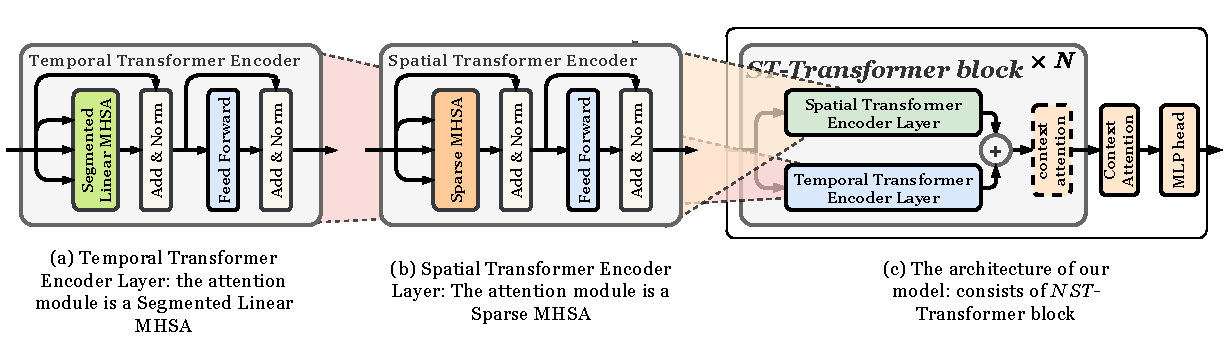
\includegraphics[width=0.95\textwidth]{architecture.pdf}
    \caption{Illustration of the overall pipeline of our approach (STAR)}
    \label{fig:arch}
\end{figure*}

\textbf{Segmented Linear Attention}. Since we concatenate the various length of video clips within a single batch along the time dimension, directly applying linear attention will cause the cross clip attention, leading to irrelevant information taken into account from one video clip to another, as shown in Figure \ref{fig:sgm_attn}. Therefore, we consider the frames of a video clip arranged as a segment, and then we design the segmented linear attention by reformulating Equation \ref{eq:lnr_attn} with segment index. Therefore, for each $V_i$ in segment $\mathcal{S}_m$, we summarize
\begin{equation}
    \begin{split}
        V_{i \in \mathcal{S}_m}' &= \frac{\phi(Q_{i \in \mathcal{S}_m})^T \sum_{j \in \mathcal{S}_m} \phi(K_{j}) V_j^T}{\phi(Q_{i \in \mathcal{S}_m})^T \sum_{j \in \mathcal{S}_m} \phi(K_j)} \\ 
        &= \frac{\phi(Q_{i \in \mathcal{S}_m})^T U_{S_m}}{\phi(Q_{i \in \mathcal{S}_m})^T Z_{S_m}} \\
        U_{S_m} &= \sum_{j \in \mathcal{S}_m} \phi(K_{j}) V_j^T, \quad Z_{S_m} = \sum_{j \in \mathcal{S}_m} \phi(K_j) 
    \end{split}
    \label{eq:sgm_lin_attn}
\end{equation}

where $\mathcal{S}_m$ is the $m$-th segment, and the reduction operation $\sum_{j \in \mathcal{S}_m} f(x)$ can be easily implemented through the indexation to segments; and with help of the gathering and scattering operations \cite{torch_scatter}, the segmented linear attention maintains the highly-paralleled computation. Figure \ref{fig:attn_ops} illustrates the comparison of different attention operations.

\subsection{STAR Framework} \label{sec:arch}

In this work, we propose the Sparse-Transformer Action Recognition (STAR) framework. Figure \ref{fig:arch} (c) shows the overview of our STAR framework. The STAR framework is built upon several Spatial-Temporal Transformer blocks (ST-block) followed by context-aware attention and MLP head for classification. Each ST-block comprises two pipelines: the spatial Transformer encoder and the temporal Transformer encoder. Each Transformer encoder consists of several key components, including the \textbf{\textit{multi-head self-attention}} (MHSA), \textbf{\textit{skip connection}} (AND \& Norm part in Figure \ref{fig:arch} (c)), and \textbf{\textit{feed-forward network}}. The spatial Transformer encoder utilizes sparse attention to capture the topological correlation of connected joints for each frame. The temporal Transformer encoder utilizes the segmented linear attention to capture the correlation of joints along the time dimension. The output sum from the two encoder layers is fed to the context-aware attention module to perform weighted summarization on the sequence of frames. Positional encoding is also utilized before ST-block to provide the context of ordering on the input sequence. Below is a brief introduction to each of them.

\subsubsection{Context-aware attention} \label{sec:context_attn}
\begin{figure}[ht]
    \centering
    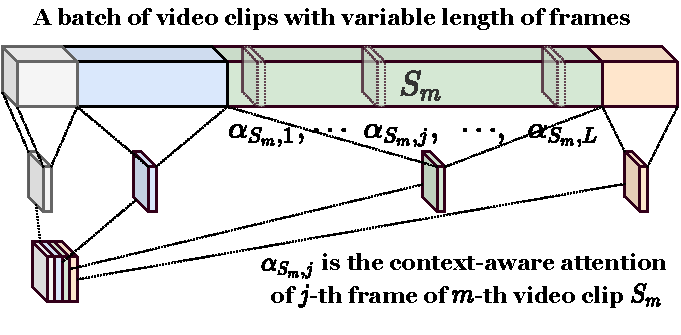
\includegraphics[width=0.45\textwidth]{context_attn.pdf}
    \caption{The context-aware attention is utilized to summarize each video clip.}
    \label{fig:context_attn}
\end{figure}

In previous works \cite{yan2018spatial, 2sagcn2019cvpr}, before connecting to the final fully-connected layer for classification, summarizing the video clip embedding along the temporal dimension is implemented by global average pooling. Alternatively, we utilize a probabilistic approach through \textit{context-aware attention}, which is extended from the work of \cite{simgnn2019}, to enhance this step's robustness, as demonstrated in Figure \ref{fig:context_attn}. Denote an input tensor embedding of video clip $S_m$ as $V \in R^{F \times N \times D}$, for $F$ is the number of frames in video clip $S_m$, $N$ is the number of joints of skeleton, and each joint possessing $D$ features, where $v_i \in R^{N \times D}$ is the embedding of frame $i$ of $V$. First, a \textit{global context} $c \in R^{N \times D}$ is computed, which is a simple average of embedding of frames followed by a nonlinear transformation: $c = tanh \left(\frac{1}{F} W \sum^{F}_{i \in S_m} v_i \right)$, where $W \in R^{D \times D}$ is a learnable weight matrix. The context $c$ provides the global structural and feature information of the video clip that is adaptive to the similarity between frames in video clip $S_m$, via learning the weight matrix. Based on $c$, we can compute one attention weight for each frame. For frame $i$, to make its attention an aware of the global context, we take the inner product between $c$ and its embedding. The intuition is that, frames similar to the global context should receive higher attention weights. A sigmoid function $\sigma(x) = \frac{1}{1 + exp(-x)}$ is applied to the result to ensure the attention weights is in the range $(0, 1)$. Finally, the video clip embedding $v' \in R^{N \times D}$ is the weighted sum of video clip embeddings, $v' = \sum^{F}_{i \in S_m} a_i v_i$. The following equations summarize the proposed context-aware attentive mechanism:
\begin{equation}
    \begin{split}
        c &= tanh \left( \frac{1}{F} W \sum^{F}_{j \in S_{m}} v_j \right) = tanh \left( \frac{1}{F} \left( V^T \cdot \mathbf{1} \right) W \right) \\
    v' &= \sum^{F}_{i \in S_m} \sigma \left( v_i^{T} \left[ tanh \left(
\frac{1}{F} W \sum^{F}_{j \in S_{m}} v_j \right) \right] \right) v_i \\
      &= \sum^{F}_{i \in S_{m}} \sigma \left( v_i^{T} c \right) v_i = \left[ \sigma (V c) \right]^T V    
    \end{split}
\end{equation}

\subsubsection{Positional Encoding} \label{sec:pos_enc}
As the attention mechanism is order-agnostic to the permutation in the input sequence \cite{attn2017all, tsai2019TransformerDissection} and treats the input as an unordered \textit{bag} of element. Therefore, an extra positional embedding is necessary to maintain the data order, i.e., time-series data are in the inherently sequential ordering. Then these positional embedding are participating the evaluation of the attention weight and value between token $i$ and $j$ in the input sequence.

\textbf{Segmented Sequential Positional Encoding}
However, as we arrange the variable-length video clips into a batch along the temporal dimension, it is not feasible to directly apply positional encoding to the whole batch. Therefore, we introduce the \textit{segmented positional encoding} where each video clip gets its positional encoding according to batch indices. An example of such encoding is shown in Figure \ref{fig:sgm_pos_enc}.

\textbf{Structural Positional Encoding}. we also attempt to apply the structural positional encoding, e.g., tree-based positional encoding \cite{neurips2019treepositional, omote-etal-2019-dependency}, to the spatial dimension, i.e., the tree topology of skeleton. Experiments show that the current approach which we used cannot improve our model's performance significantly. Hence, to reduce our model's complexity, we decide not to apply the structural positional encoding for this work and leave it for future research.

\begin{figure}[ht]
    \centering
    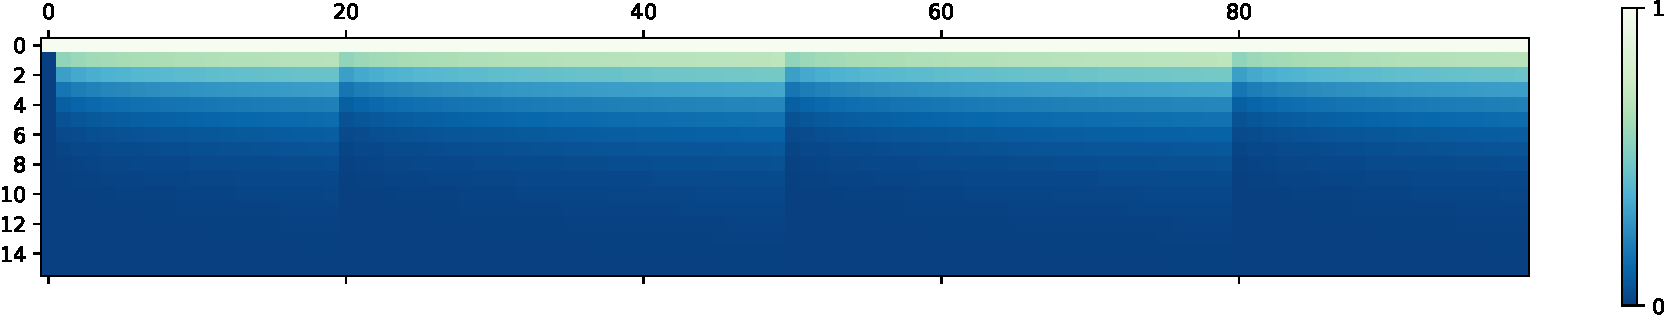
\includegraphics[width=0.47\textwidth]{sgm_pos_enc.pdf}
    \caption{Illustration of Segmented Positional Encoding for a batch of 4 video clips. x-axis represents the number of frames and y-axis represents the feature dimension.}
    \label{fig:sgm_pos_enc}
\end{figure}

% ----------------------- Experiment -------------------------
\begin{table*}[h!]
\centering
\begin{tabular}{ccccc}
       & \multicolumn{2}{c}{NTU-60}  & \multicolumn{2}{c}{NTU-120} \\ 
\toprule \textbf{Method} & \textbf{X-subject} & \textbf{X-view} & \textbf{X-subject} & \textbf{X-setup} \\ 
\hline
ST-GCN & 81.5 & 88.3 & 72.4& 71.3\\
ST-TR & 88.7 & 95.6 & 81.9.& 84.1\\
STAR-64 (ours) & 81.9 & 88.9 & 75.4& 78.1\\ 
STAR-128 (ours) & 83.4 & 89.0 & 78.3& 80.2\\
\hline
\end{tabular}
\caption{Comparison of models' accuracy on NTU RGB+D 60 and 120 datasets}
\label{tab:accuracy}
\end{table*}

\begin{table*}[!h]
\centering
\begin{tabular}{cccc}
\hline
\textbf{Model}    & \textbf{CUDA time (ms)} & \textbf{num. of parameters} & \textbf{GMACs}\\ \hline
ST-GCN   & 333.89  & 3.1M               & 261.49\\
ST-TR    & 1593.05  & 6.73M              & 197.55\\
STAR-64 (ours)  & 86.54   & 0.42M              & 15.58\\
STAR-128 (ours) & 191.23    & 1.26M             & 73.33\\ \hline
\end{tabular}
\caption{Comparison of models' efficiency}
\label{tab:efficiency}
\end{table*}

\section{Experiments}
In this section, we conduct experiments and ablation studies to verify the effectiveness and efficiency of our proposed sparse spatial and segmented linear temporal self-attention operations. The comparison has been made with \textbf{ST-GCN}, the baseline GCN model, and \textbf{ST-TR}, one of the state-of-the-art hybrid model, which have utilized full attention operation coupled with graph convolutions. The corresponding analysis demonstrates the potential of our model and the possible room for improvements.

\subsection{Datasets}
In the experiments, we evaluate our model on two largest scale 3D skeleton-based action recognition datasets, NTU-RGB+D 60 and 120. 
\subsubsection{NTU RGB+D 60}
This dataset contains 56,880 video clips involving 60 human action classes. The samples are performed by 40 volunteers and captured by three Microsoft Kinect v2 cameras \cite{shahroudy2016ntu}. It contains four modalities, including RGB videos, depth sequences, infrared frames, and 3D skeleton data. Our experiments are only conducted with the 3D skeleton data. The length of the action samples vary from 32 frames to 300 frames. In each frame, there are at most 2 subjects and each subject contains 25 3D joint coordinates. The dataset follows two evaluation criteria, which are Cross-Subject and Cross-View. In the Cross-View evaluation (X-View), there are 37,920 training samples captured from camera 2 and 3 and 18,960 test samples captured from camera 1. In the Cross-Subject evaluation (X-Sub), there are 40,320 training samples from 20 subjects and 26,560 test samples from the rest. We follow the original two benchmarks and report the Top-1 accuracy as well as the profiling metrics.
\subsubsection{NTU RGB+D 120}
The dataset \cite{liu2019ntu} extends from NTU RGB+D 60 and is currently the largest dataset with 3D joint annotations. It contains 57,600 new skeleton sequences representing 60 new actions, a total of 114,480 videos involving 120 classes of 106 subjects captured from 32 different camera setups. The dataset follows two criteria, which are Cross-Subject and Cross-Setup. In the Cross-Subject evaluation, similar to the previous dataset, splits subjects in half to training and testing dataset. In the Cross-Setup evaluation, the samples are divided by the 32 camera setup IDs, where the even setup IDs are for training and the odd setup IDs for testing. Similar to the previous dataset, there is no preprocessing to set the uniform video length for all the samples. We follow the two criteria and report the Top-1 accuracy and the profiling metrics.

Unlike GCN-based models, where the length of all the samples and the number of subjects need to be fixed (e.g. 300 frames and 2 subjects), our model can process varying length of input samples and of the number of subjects. So no further preprocessing with padding is done on the samples.

\subsection{Configuration of experiments}
\textbf{Implementation details}. As the original Transformer framework \cite{attn2017all} employs the unified model size $d$ for every layer, we follow the same notion and keep the hidden channel size uniform across the attention heads and the feedforward networks. We run the experiments with two different hidden channel sizes, 64 and 128 for our Transformer encoders (STAR-64 and STAR-128), respectively. The hidden channel size of the MLP head is also proportional to that of the attention heads. Our model consists of 5 layers, each layer comprises one spatial encoder and one temporal encoder in parallel and the  output sum from the two encoders is fed to the next layer. Drop rates are set to 0.5 for every module. We also replace the ReLU non-linear activation funciton with SiLU (or Swish) \cite{elfwing2018sigmoid, swish2017} to increase the stability of gradients in back-propagation phase (GELU or SELU also bring similar effect). Our model is implemented with the deep learning framework PyTorch \cite{pytorch} and its extension PyTorch Geometric \cite{pytorch_geometric_Fey2019}. The scattering/gathering operations and sparse matrix multiplications are based on PyTorch Scatter \cite{torch_scatter} and PyTorch Sparse \cite{torch_sparse}, respectively.

\begin{table*}[!h]
\centering
\begin{tabular}{cccc}
    & \textbf{MACs} & \textbf{Parameters} & \textbf{Latency} \\ \toprule %hline
    ST-GCN & 
    \begin{tabular}[l]{@{}l@{}}
       \textit{Conv2d}: 260.4 GMACs \\ 
       \textit{BatchNorm2d}: 737.3 MMACs \\ 
       \textit{ReLU}: 184.3 MMACs
    \end{tabular} & 
    \begin{tabular}[l]{@{}l@{}}
       \textit{Conv2d}: 3.06M \\ 
       \textit{BatchNorm2d}: 6.4K \\ 
       \textit{Linear}: 15.4K 
    \end{tabular} & 
    \begin{tabular}[l]{@{}l@{}}
       \textit{Conv2d}: 149.92ms \\ 
       \textit{BatchNorm2d}: 19.92ms \\ 
       \textit{ReLU}: 4.49ms
    \end{tabular} \\ \hline

    ST-TR  & 
    \begin{tabular}[l]{@{}l@{}}
       \textit{Conv2d}: 810.57 GMACs \\ 
       \textit{MatMul}: 161.1 GMACs \\ 
       \textit{BatchNorm2d}: 138.4 MMACs
    \end{tabular}  & 
    \begin{tabular}[l]{@{}l@{}}
       \textit{Conv2d}: 2.7M \\ 
       \textit{BatchNorm2d}: 10.5K \\ 
       \textit{Linear}: 30.8K
    \end{tabular} & 
    \begin{tabular}[l]{@{}l@{}}
       \textit{Conv2d}: 692.39ms \\ 
       \textit{MatMul}: 161.38ms \\ 
       \textit{BatchNorm2d}: 38.97ms
    \end{tabular} \\ \hline

    STAR-64   & 
    \begin{tabular}[l]{@{}l@{}}
       MatMul(attention): 24.4 GMACs\\
       Mul(sparse): 12.3 GMACs \\
       Linear: 6.2 GMACs
    \end{tabular} & 
    \begin{tabular}[l]{@{}l@{}}
    Linear:83.2K\\
    LayerNorm: 1.3K
    \end{tabular} & 
    \begin{tabular}[l]{@{}l@{}}
       MatMul: 25.27ms \\
       Mul: 12.81ms\\
       Linear:6.53ms
    \end{tabular}   \\ \hline

\end{tabular}
\caption{The breakdown analysis and top-3 components in each metrics}
\label{tab:3_metrics}
\end{table*}

\textbf{Training setting}. The maximum number of training epochs is set to 100. We used the Adam optimizer \cite{kingma2014adam} with $\beta_1 = 0.9$, $\beta_2 = 0.98$ and $\epsilon = 10^{-9}$. Following the setting of the original Transformer paper \cite{attn2017all}, the learning rate is adjusted throughout the training:
\begin{equation}
    lrate = d^{-0.5} \cdot min(t^{-0.5}, t \cdot w^{-1.5})
    \label{eq:warmup}
\end{equation}
where $d$ is the model dimension, $s$ is \textit{step number}, and $w$ is the \textit{warmup steps}. According to the equation \ref{eq:warmup}, the learning rate linearly increases for the first $w$ training steps and then decreases proportionally to the inverse square root of the step number. We keep the original settings for the baseline models in their papers \cite{yan2018spatial, plizzari2020spatial}, and use their codes provided online. 
All our training experiments are performed on a system with two GTX TITAN X GPUs and a system with one TITAN RTX GPU, while the inferences are executed on a single GPU. % TODO: verify

\subsection{Results and Analysis}
We evaluate the accuracy and the efficiency of the baseline GCN model (ST-GCN), our model (STAR) and the hybrid model (ST-TR), which utilize both transformer and GCN frameworks.

\subsubsection{Accuracy}
We first evaluate the effectiveness of our Transformer encoder based model compared to ST-TR and ST-GCN models. Each model's accuracy is evaluated with the NTU RGB+D 60 and 120 testing datasets. As shown in the Table \ref{tab:accuracy}, our model outperforms ST-GCN in both cross-view (cross-set) and cross-subject benchmarks of the two dataset. Our model achieves 3.6 $\sim$ 7.7 percent lower accuracy compared to ST-TR, which heavily relies on convolution-based key components inherited from ST-GCN and utilizes them in both spatial and temporal pipelines. Our model yields modest performance compared to the state-of-the-art models in NTU RGB+D 60 and 120 when trained from scratch. The Figure \ref{fig:general} shows that there exists a performance gap between the training and testing. Transformer architectures' lack of inductive biases, especially translation equivariance and locality that are essential to convolution networks, could result in weak generalization. In NLP, Transformers are usually pretrained on a large corpus of text and fine-tuned on a smaller task-specific dataset to boost the performance. We would like to conduct extensive experiments on pre-training and fine-tuning our model on a larger dataset in the future to improve the accuracy comparable to those of the state-of-the-art models. For our future study, we want to address effective generalization methods for Transformer models, which resolves overfitting issues and improve the overall performance.

\subsubsection{Efficiency} 
In this section, we evaluate the efficiency of the different models. As shown in Table \ref{tab:efficiency}, our model (STAR) is significantly efficient in terms of model size, the number of multiply-accumulate operations (GMACs) and the latency. Each metric for the different models is evaluated by running inference with sample dataset. Our model is fed with the original skeleton sequence of varying length. The other two models are fed with fix-sized skeleton sequence padded to 300 frames and 2 persons. We use the official profiler of PyTorch (v1.8.1) \cite{pytorch}, and Flops-Profiler of DeepSpeed \cite{deepspeed2020kdd} to measure the benchmarks. The results are summarized with the following metrics:
\begin{figure*}[h!]
    \centering
    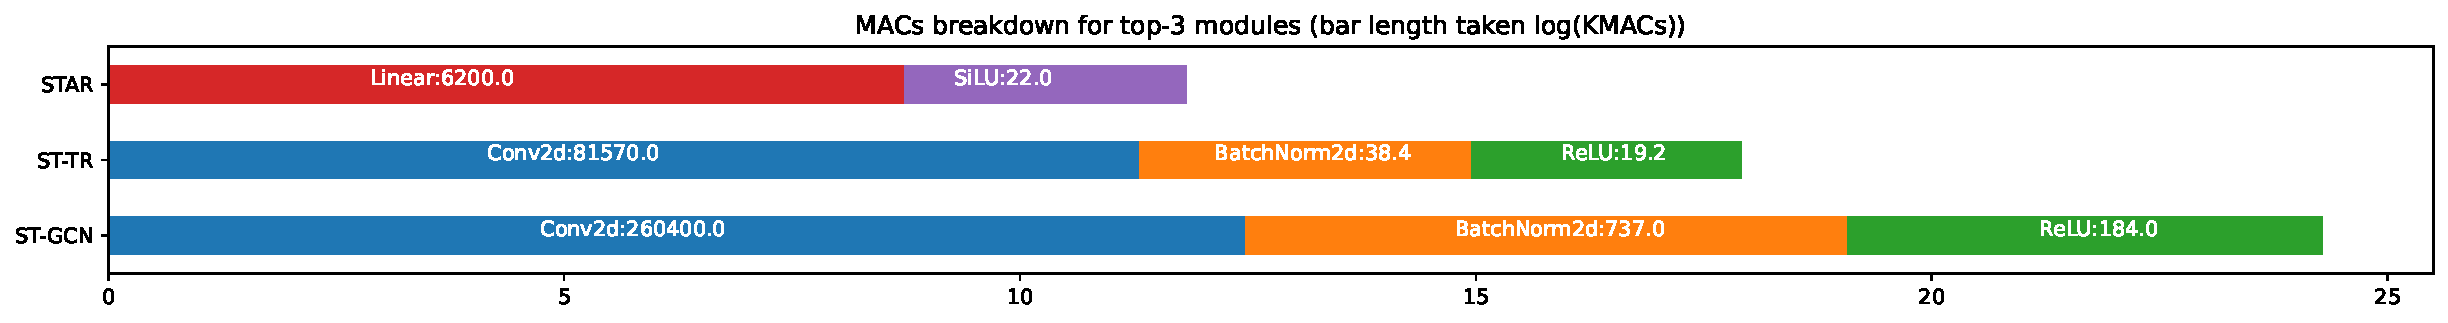
\includegraphics[width=0.84\textwidth]{mac_breakdown.pdf}
    \caption{The breakdown of MACs for top-3 modules}
    \label{fig:mac_breakdown}
\end{figure*}

\begin{figure*}[h!]
    \centering
    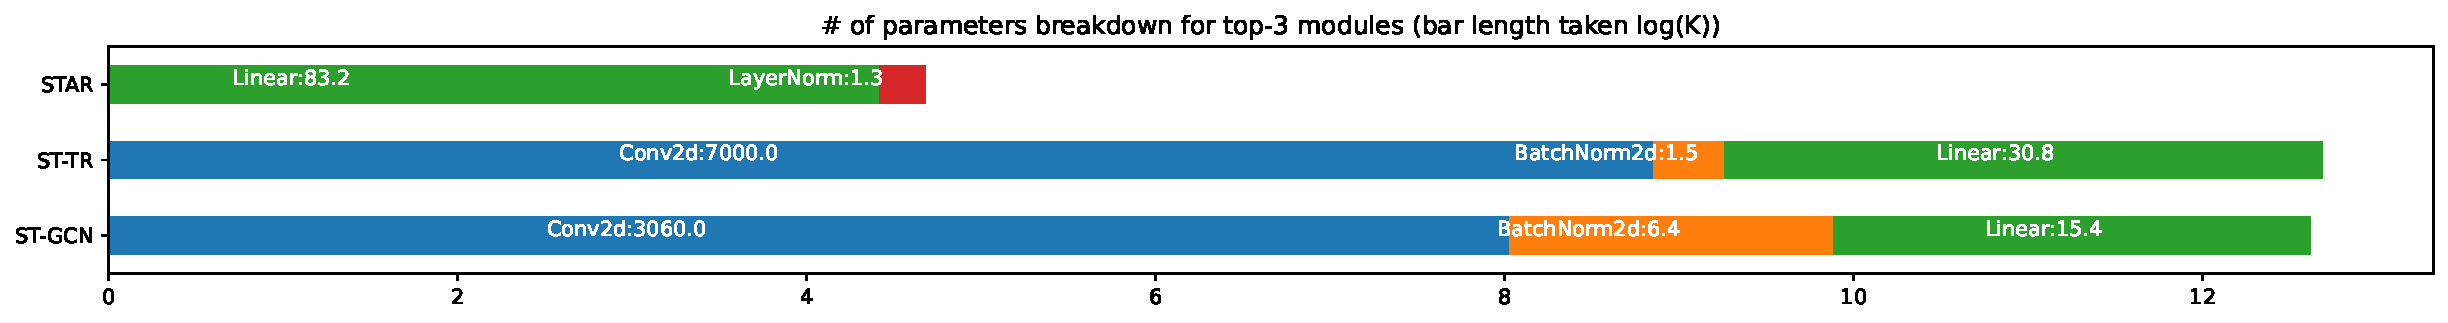
\includegraphics[width=0.84\textwidth]{params_breakdown.pdf}
    \caption{The breakdown of \# parameters for top-3 modules} \label{fig:param_breakdown}
\end{figure*}

\begin{figure*}[h!]
    \centering
    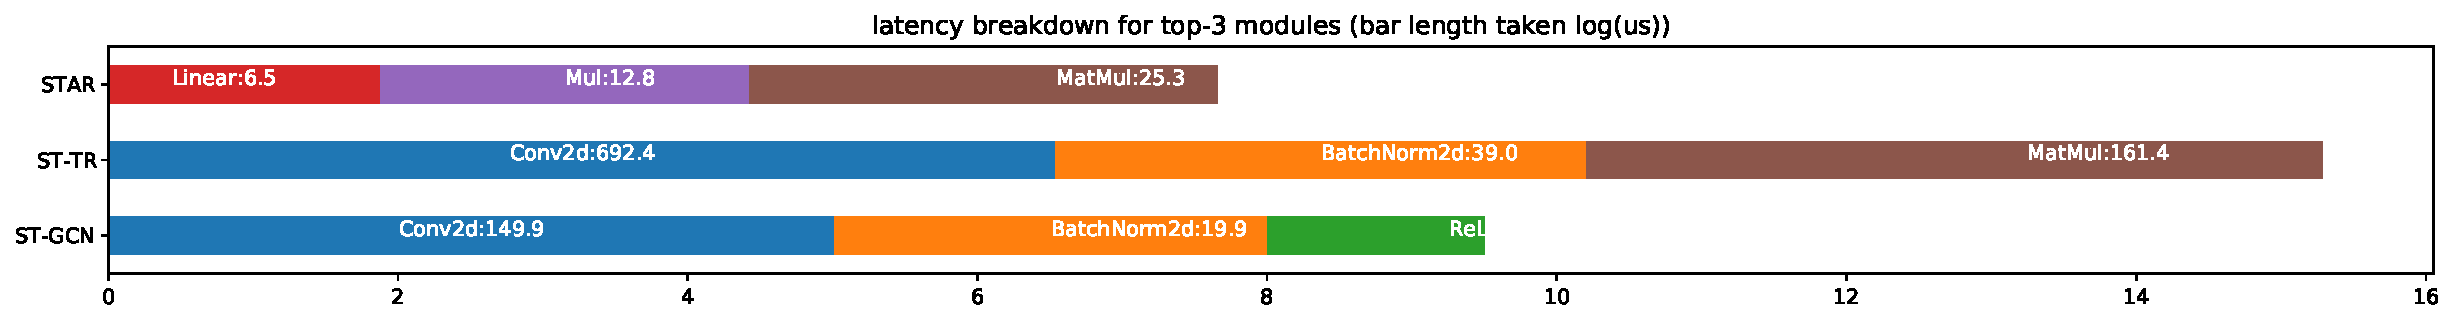
\includegraphics[width=0.84\textwidth]{latency_breakdown.pdf}
    \caption{The breakdown of latency for top-3 modules}
    \label{fig:latency_breakdown}
\end{figure*}

\textbf{MACs}. The number of Multiply-Accumulate (MAC) operations is used to determine the efficiency of deep learning models. Each MAC operation is counted as two floating point operations. With the same hardware configuration, more efficient models require fewer MACs than other models to fulfill the same task. As shown in Table \ref{tab:efficiency}, both of our model with different channel sizes execute only $\frac{1}{3} \sim \frac{1}{17}$ amount of GMACs (i.e., Giga MACs) compared to ST-GCN and ST-TR models, respectively.

\textbf{Model size}. Model size is another metric to measure the efficiency of a machine learning model. Given the same task, smaller model delivering the same or very close performance is preferable. Smaller model is not only beneficial for the higher speedup and less memory accesses but also gives better energy consumption, especially for embedded systems and edge devices with scarce computational resources and small storage volume. The column of the number of parameters in Table \ref{tab:efficiency} depicts the size of the models, these parameters are trainable weights in the model. Among all the model, STAR possesses the smallest model size,  0.42M and 1.26M for STAT-64 and STAR-128, respectively.

\begin{figure*}[h!]
    \centering
    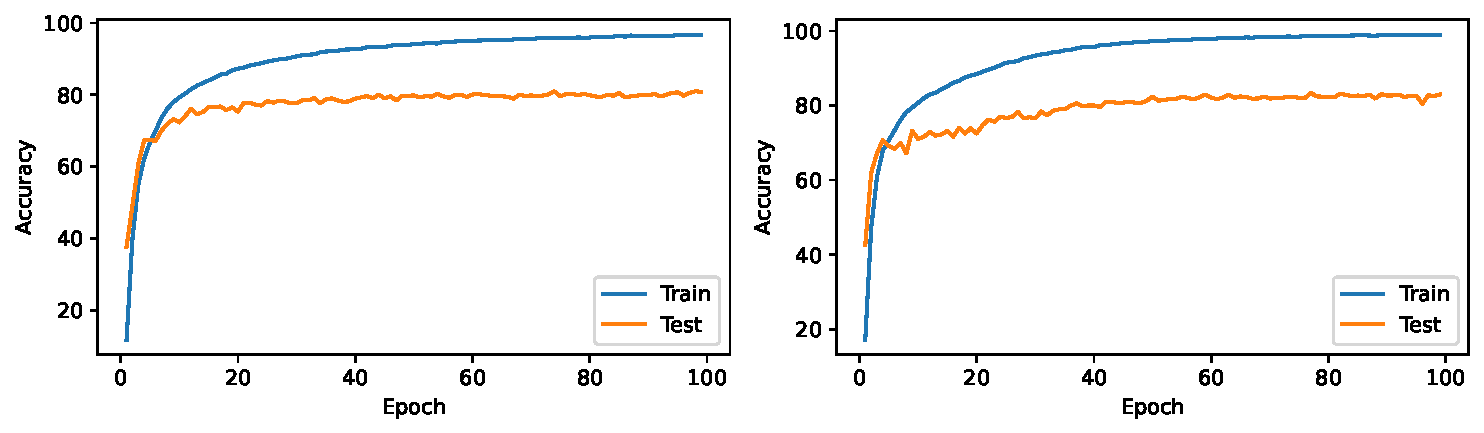
\includegraphics[width=.76\textwidth]{graph.pdf}
    \caption{The training and testing curve for STAR-64(left) and STAR-128(right) on NTU-RGB+D 60 X-subject benchmark.}
    \label{fig:general}
\end{figure*}

\textbf{Breakdown analysis}.
The breakdown analysis is used to identify potential bottlenecks within different models (STAR-64, ST-TR, and ST-GCN). Table \ref{tab:3_metrics} provides the detailed profiling results for the top-3 computation modules that are dominant in each models. According to Figure \ref{fig:mac_breakdown}, \ref{fig:param_breakdown} and \ref{fig:latency_breakdown}, the convolution operations cost significant number of MAC operations and lead to computation bound. ST-GCN and ST-TR mainly consist of the convolution operations followed by batch normalization, which requires relatively large computational resources. Our Transformer model is based on sparse and linear attention mechanisms. It only produces relatively small attention weights from sparse attention; and performs low-rank matrix multiplication for linear attention ($\mathcal{O}(n)$). This replaces huge dynamic weights of attention coefficients from the standard attention mechanism, which has a quadratic time and space complexity ($\mathcal{O}(n^2)$). 

\subsection{Ablation Study}.
In this section, we evaluate the effectiveness and efficiency of our sparse self-attention operation in spatial encoder compared to the standard transformer encoder with full-attention operation. Table \ref{tab:acc_ablation} and Table \ref{tab:eff_ablation} show that our model with sparse self-attention operation achieves higher accuracy on both X-subject and X-view benchmarks and use significantly less number of GMACs and runtime. This shows that additional correlations of distant joints calculated by full attention do not improve the performance but rather contribute noise to the prediction. To handle such issue, learnable masks, consistent with adjacency matrix of skeleton, can be integrated to the full attention calculation to avoid accuracy degradation. But it requires extra computation involving learnable masks. 

\begin{table}[h!]
\centering
\begin{tabular}{ccccc}
       & \multicolumn{2}{c}{NTU-60}  & \multicolumn{2}{c}{NTU-120} \\ 
\toprule Method & X-subject & X-view & X-subject & X-setup \\ 
\hline
    STAR (sparse) & 83.4&84.2 & 78.3& 78.5 \\
    STAR (full) & 80.7&81.9 & 77.4& 77.7 \\
\hline
\end{tabular}
    \caption{Classification accuracy comparison between Sparse attention and Full attention on the NTU RGB+D 60 Skeleton dataset.}
\label{tab:acc_ablation}
\end{table}

\begin{table}[!h]
\centering
\begin{tabular}{ccccc}
\hline
Model    & CUDA time (ms) & GMACs  \\ \hline
STAR-sparse  & 105.7   & 15.58 \\
STAR-full & 254.7      & 73.33    \\ \hline
\end{tabular}
\caption{Efficiency comparison between Sparse attention and Full attention on the NTU RGB+D 60 Skeleton dataset.}
\label{tab:eff_ablation}
\end{table}

% ----------------------- Conclusion --------------------------

\section{Conclusion}
In this paper, we propose an efficient Transformer-based model with sparse attention and segmented linear attention mechanisms applied on spatial and temporal dimensions of action skeleton sequence. We demonstrate that our model can replace graph convolution operations with the self-attention operations and yield the modest performance, while requiring significantly less computational and memory resources. We also designed compact data representation which is much smaller than fixed-size and zero padded data representation utilized by previous models. This work was supported in part by Semiconductor Research Corporation (SRC).
 
%%%%%%%%%%%%%%%%%%%%%%%%% References %%%%%%%%%%%%%%%%%%%%%%%%%

%\bibliographystyle{unsrt}
\bibliography{references.bib}

% \noindent Congratulations on having a paper selected for inclusion in an AAAI Press proceedings or technical report! This document details the requirements necessary to get your accepted paper published using PDF\LaTeX{}. If you are using Microsoft Word, instructions are provided in a different document. AAAI Press does not support any other formatting software.

% The instructions herein are provided as a general guide for experienced \LaTeX{} users. If you do not know how to use \LaTeX{}, please obtain assistance locally. AAAI cannot provide you with support and the accompanying style files are \textbf{not} guaranteed to work. If the results you obtain are not in accordance with the specifications you received, you must correct your source file to achieve the correct result.

% These instructions are generic. Consequently, they do not include specific dates, page charges, and so forth. Please consult your specific written conference instructions for details regarding your submission. Please review the entire document for specific instructions that might apply to your particular situation. All authors must comply with the following:

% \begin{itemize}
% \item You must use the 2021 AAAI Press \LaTeX{} style file and the aaai21.bst bibliography style files, which are located in the 2021 AAAI Author Kit (aaai21.sty, aaai21.bst).
% \item You must complete, sign, and return by the deadline the AAAI copyright form (unless directed by AAAI Press to use the AAAI Distribution License instead).
% \item You must read and format your paper source and PDF according to the formatting instructions for authors.
% \item You must submit your electronic files and abstract using our electronic submission form \textbf{on time.}
% \item You must pay any required page or formatting charges to AAAI Press so that they are received by the deadline.
% \item You must check your paper before submitting it, ensuring that it compiles without error, and complies with the guidelines found in the AAAI Author Kit.
% \end{itemize}

% \section{Copyright}
% All papers submitted for publication by AAAI Press must be accompanied by a valid signed copyright form. They must also contain the AAAI copyright notice at the bottom of the first page of the paper. There are no exceptions to these requirements. If you fail to provide us with a signed copyright form or disable the copyright notice, we will be unable to publish your paper. There are \textbf{no exceptions} to this policy. You will find a PDF version of the AAAI copyright form in the AAAI AuthorKit. Please see the specific instructions for your conference for submission details.

% \section{Formatting Requirements in Brief}
% We need source and PDF files that can be used in a variety of ways and can be output on a variety of devices. The design and appearance of the paper is strictly governed by the aaai style file (aaai21.sty).
% \textbf{You must not make any changes to the aaai style file, nor use any commands, packages, style files, or macros within your own paper that alter that design, including, but not limited to spacing, floats, margins, fonts, font size, and appearance.} AAAI imposes requirements on your source and PDF files that must be followed. Most of these requirements are based on our efforts to standardize conference manuscript properties and layout. All papers submitted to AAAI for publication will be recompiled for standardization purposes. Consequently, every paper submission must comply with the following requirements:

% \begin{quote}
% \begin{itemize}
% \item Your .tex file must compile in PDF\LaTeX{} --- (you may not include .ps or .eps figure files.)
% \item All fonts must be embedded in the PDF file --- including includes your figures.
% \item Modifications to the style file, whether directly or via commands in your document may not ever be made, most especially when made in an effort to avoid extra page charges or make your paper fit in a specific number of pages.
% \item No type 3 fonts may be used (even in illustrations).
% \item You may not alter the spacing above and below captions, figures, headings, and subheadings.
% \item You may not alter the font sizes of text elements, footnotes, heading elements, captions, or title information (for references and mathematics, please see the limited exceptions provided herein).
% \item You may not alter the line spacing of text.
% \item Your title must follow Title Case capitalization rules (not sentence case).
% \item Your .tex file must include completed metadata to pass-through to the PDF (see PDFINFO below).
% \item \LaTeX{} documents must use the Times or Nimbus font package (you may not use Computer Modern for the text of your paper).
% \item No \LaTeX{} 209 documents may be used or submitted.
% \item Your source must not require use of fonts for non-Roman alphabets within the text itself. If your paper includes symbols in other languages (such as, but not limited to, Arabic, Chinese, Hebrew, Japanese, Thai, Russian and other Cyrillic languages), you must restrict their use to bit-mapped figures. Fonts that require non-English language support (CID and Identity-H) must be converted to outlines or 300 dpi bitmap or removed from the document (even if they are in a graphics file embedded in the document).
% \item Two-column format in AAAI style is required for all papers.
% \item The paper size for final submission must be US letter without exception.
% \item The source file must exactly match the PDF.
% \item The document margins may not be exceeded (no overfull boxes).
% \item The number of pages and the file size must be as specified for your event.
% \item No document may be password protected.
% \item Neither the PDFs nor the source may contain any embedded links or bookmarks (no hyperref or navigator packages).
% \item Your source and PDF must not have any page numbers, footers, or headers (no pagestyle commands).
% \item Your PDF must be compatible with Acrobat 5 or higher.
% \item Your \LaTeX{} source file (excluding references) must consist of a \textbf{single} file (use of the ``input" command is not allowed.
% \item Your graphics must be sized appropriately outside of \LaTeX{} (do not use the ``clip" or ``trim'' command) .
% \end{itemize}
% \end{quote}

% If you do not follow these requirements, your paper will be returned to you to correct the deficiencies.

% \section{What Files to Submit}
% You must submit the following items to ensure that your paper is published:
% \begin{itemize}
% \item A fully-compliant PDF file that includes PDF metadata.
% \item Your \LaTeX{} source file submitted as a \textbf{single} .tex file (do not use the ``input" command to include sections of your paper --- every section must be in the single source file). (The only allowable exception is .bib file, which should be included separately).
% \item The bibliography (.bib) file(s).
% \item Your source must compile on our system, which includes only standard \LaTeX{} 2020 TeXLive support files.
% \item Only the graphics files used in compiling paper.
% \item The \LaTeX{}-generated files (e.g. .aux,  .bbl file, PDF, etc.).
% \end{itemize}

% Your \LaTeX{} source will be reviewed and recompiled on our system (if it does not compile, your paper will be returned to you. \textbf{Do not submit your source in multiple text files.} Your single \LaTeX{} source file must include all your text, your bibliography (formatted using aaai21.bst), and any custom macros.

% Your files should work without any supporting files (other than the program itself) on any computer with a standard \LaTeX{} distribution.

% \textbf{Do not send files that are not actually used in the paper.} We don't want you to send us any files not needed for compiling your paper, including, for example, this instructions file, unused graphics files, style files, additional material sent for the purpose of the paper review, and so forth.

% \textbf{Do not send supporting files that are not actually used in the paper.} We don't want you to send us any files not needed for compiling your paper, including, for example, this instructions file, unused graphics files, style files, additional material sent for the purpose of the paper review, and so forth.

% \textbf{Obsolete style files.} The commands for some common packages (such as some used for algorithms), may have changed. Please be certain that you are not compiling your paper using old or obsolete style files.

% \textbf{Final Archive.} Place your PDF and source files in a single archive which should be compressed using .zip. The final file size may not exceed 10 MB.
% Name your source file with the last (family) name of the first author, even if that is not you.


% \section{Using \LaTeX{} to Format Your Paper}

% The latest version of the AAAI style file is available on AAAI's website. Download this file and place it in the \TeX\ search path. Placing it in the same directory as the paper should also work. You must download the latest version of the complete AAAI Author Kit so that you will have the latest instruction set and style file.

% \subsection{Document Preamble}

% In the \LaTeX{} source for your paper, you \textbf{must} place the following lines as shown in the example in this subsection. This command set-up is for three authors. Add or subtract author and address lines as necessary, and uncomment the portions that apply to you. In most instances, this is all you need to do to format your paper in the Times font. The helvet package will cause Helvetica to be used for sans serif. These files are part of the PSNFSS2e package, which is freely available from many Internet sites (and is often part of a standard installation).

% Leave the setcounter for section number depth commented out and set at 0 unless you want to add section numbers to your paper. If you do add section numbers, you must uncomment this line and change the number to 1 (for section numbers), or 2 (for section and subsection numbers). The style file will not work properly with numbering of subsubsections, so do not use a number higher than 2.

% \subsubsection{The Following Must Appear in Your Preamble}
% \begin{quote}
% \begin{scriptsize}\begin{verbatim}
% \def\year{2021}\relax
% % File: formatting-instruction.tex
% \documentclass[letterpaper]{article}
% % DO NOT CHANGE THIS
% \usepackage{aaai21} % DO NOT CHANGE THIS
% \usepackage{times} % DO NOT CHANGE THIS
% \usepackage{helvet} % DO NOT CHANGE THIS
% \usepackage{courier} % DO NOT CHANGE THIS
% \usepackage[hyphens]{url} % DO NOT CHANGE THIS
% \usepackage{graphicx} % DO NOT CHANGE THIS
% \urlstyle{rm} % DO NOT CHANGE THIS
% \def\UrlFont{\rm} % DO NOT CHANGE THIS
% \usepackage{graphicx}  % DO NOT CHANGE THIS
% \usepackage{natbib}
% % DO NOT CHANGE THIS OR ADD OPTIONS
% \usepackage{caption}
% % DO NOT CHANGE THIS OR ADD OPTIONS
% \frenchspacing % DO NOT CHANGE THIS
% \setlength{\pdfpagewidth}{8.5in} % DO NOT CHANGE THIS
% \setlength{\pdfpageheight}{11in} % DO NOT CHANGE THIS
% %
% % PDF Info Is REQUIRED.
% % For /Author, add all authors within the parentheses,
% % separated by commas. No accents or commands.
% % For /Title, add Title in Mixed Case.
% % No accents or commands. Retain the parentheses.
% \pdfinfo{
% /Title (AAAI Press Formatting Instructions for Authors
% Using LaTeX -- A Guide)
% /Author (AAAI Press Staff, Pater Patel Schneider,
% Sunil Issar, J. Scott Penberthy, George Ferguson,
% Hans Guesgen, Francisco Cruz, Marc Pujol-Gonzalez)
% /TemplateVersion (2021.1)
% }
% \end{verbatim}\end{scriptsize}
% \end{quote}

% \subsection{Preparing Your Paper}

% After the preamble above, you should prepare your paper as follows:
% \begin{quote}
% \begin{scriptsize}\begin{verbatim}
% %
% \begin{document}
% \maketitle
% \begin{abstract}
% %...
% \end{abstract}\end{verbatim}\end{scriptsize}
% \end{quote}

% \noindent You should then continue with the body of your paper. Your paper must conclude with the references, which should be inserted as follows:
% \begin{quote}
% \begin{scriptsize}\begin{verbatim}
% % References and End of Paper
% % These lines must be placed at the end of your paper
% \bibliography{Bibliography-File}
% \end{document}
% \end{verbatim}\end{scriptsize}
% \end{quote}

% \subsection{Inserting Document Metadata with \LaTeX{}}
% PDF files contain document summary information that enables us to create an Acrobat index (pdx) file, and also allows search engines to locate and present your paper more accurately. \textit{Document metadata for author and title are REQUIRED.} You may not apply any script or macro to implementation of the title, author, and metadata information in your paper.

% \textit{Important:} Do not include \textit{any} \LaTeX{} code or nonascii characters (including accented characters) in the metadata. The data in the metadata must be completely plain ascii. It may not include slashes, accents, linebreaks, unicode, or any \LaTeX{} commands. Type the title exactly as it appears on the paper (minus all formatting). Input the author names in the order in which they appear on the paper (minus all accents), separating each author by a comma. You may also include keywords in the optional Keywords field.

% \begin{quote}
% \begin{scriptsize}\begin{verbatim}
% \begin{document}\\
% \maketitle\\
% ...\\
% \bibliography{Bibliography-File}\\
% \end{document}\\
% \end{verbatim}\end{scriptsize}
% \end{quote}

% \subsection{Commands and Packages That May Not Be Used}
% \begin{table*}[t]
% \centering

% \begin{tabular}{l|l|l|l}
% \textbackslash abovecaption &
% \textbackslash abovedisplay &
% \textbackslash addevensidemargin &
% \textbackslash addsidemargin \\
% \textbackslash addtolength &
% \textbackslash baselinestretch &
% \textbackslash belowcaption &
% \textbackslash belowdisplay \\
% \textbackslash break &
% \textbackslash clearpage &
% \textbackslash clip &
% \textbackslash columnsep \\
% \textbackslash float &
% \textbackslash input &
% \textbackslash input &
% \textbackslash linespread \\
% \textbackslash newpage &
% \textbackslash pagebreak &
% \textbackslash renewcommand &
% \textbackslash setlength \\
% \textbackslash text height &
% \textbackslash tiny &
% \textbackslash top margin &
% \textbackslash trim \\
% \textbackslash vskip\{- &
% \textbackslash vspace\{- \\
% \end{tabular}
% %}
% \caption{Commands that must not be used}
% \label{table1}
% \end{table*}

% \begin{table}[t]
% \centering
% %\resizebox{.95\columnwidth}{!}{
% \begin{tabular}{l|l|l|l}
%     authblk & babel & cjk & dvips \\
%     epsf & epsfig & euler & float \\
%     fullpage & geometry & graphics & hyperref \\
%     layout & linespread & lmodern & maltepaper \\
%     navigator & pdfcomment & pgfplots & psfig \\
%     pstricks & t1enc & titlesec & tocbind \\
%     ulem
% \end{tabular}
% \caption{LaTeX style packages that must not be used.}
% \label{table2}
% \end{table}

% There are a number of packages, commands, scripts, and macros that are incompatable with aaai21.sty. The common ones are listed in tables \ref{table1} and \ref{table2}. Generally, if a command, package, script, or macro alters floats, margins, fonts, sizing, linespacing, or the presentation of the references and citations, it is unacceptable. Note that negative vskip and vspace may not be used except in certain rare occurances, and may never be used around tables, figures, captions, sections, subsections, subsections, or references.


% \subsection{Page Breaks}
% For your final camera ready copy, you must not use any page break commands. References must flow directly after the text without breaks. Note that some conferences require references to be on a separate page during the review process. AAAI Press, however, does not require this condition for the final paper.


% \subsection{Paper Size, Margins, and Column Width}
% Papers must be formatted to print in two-column format on 8.5 x 11 inch US letter-sized paper. The margins must be exactly as follows:
% \begin{itemize}
% \item Top margin: .75 inches
% \item Left margin: .75 inches
% \item Right margin: .75 inches
% \item Bottom margin: 1.25 inches
% \end{itemize}


% The default paper size in most installations of \LaTeX{} is A4. However, because we require that your electronic paper be formatted in US letter size, the preamble we have provided includes commands that alter the default to US letter size. Please note that using any other package to alter page size (such as, but not limited to the Geometry package) will result in your final paper being returned to you for correction.


% \subsubsection{Column Width and Margins.}
% To ensure maximum readability, your paper must include two columns. Each column should be 3.3 inches wide (slightly more than 3.25 inches), with a .375 inch (.952 cm) gutter of white space between the two columns. The aaai21.sty file will automatically create these columns for you.

% \subsection{Overlength Papers}
% If your paper is too long and you resort to formatting tricks to make it fit, it is quite likely that it will be returned to you. The best way to retain readability if the paper is overlength is to cut text, figures, or tables. There are, a few acceptable ways to reduce paper size that don't affect readability. First, turn on \textbackslash frenchspacing, which will reduce the space after periods. Next, move all your figures and tables to the top of the page. Consider removing less important portions of a figure. If you use \textbackslash centering instead of \textbackslash begin\{center\} in your figure environment, you can also buy some space. For mathematical environments, you may reduce fontsize {\bf but not below 6.5 point}.


% Commands that alter page layout are forbidden. These include \textbackslash columnsep,  \textbackslash float, \textbackslash topmargin, \textbackslash topskip, \textbackslash textheight, \textbackslash textwidth, \textbackslash oddsidemargin, and \textbackslash evensizemargin (this list is not exhaustive). If you alter page layout, you will be required to pay the page fee. Other commands that are questionable and may cause your paper to be rejected include \textbackslash parindent, and \textbackslash parskip. Commands that alter the space between sections are forbidden. The title sec package is not allowed. Regardless of the above, if your paper is obviously ``squeezed" it is not going to to be accepted. Options for reducing the length of a paper include reducing the size of your graphics, cutting text, or paying the extra page charge (if it is offered).


% \subsection{Type Font and Size}
% Your paper must be formatted in Times Roman or Nimbus. We will not accept papers formatted using Computer Modern or Palatino or some other font as the text or heading typeface. Sans serif, when used, should be Courier. Use Symbol or Lucida or Computer Modern for \textit{mathematics only. }

% Do not use type 3 fonts for any portion of your paper, including graphics. Type 3 bitmapped fonts are designed for fixed resolution printers. Most print at 300 dpi even if the printer resolution is 1200 dpi or higher. They also often cause high resolution imagesetter devices to crash. Consequently, AAAI will not accept electronic files containing obsolete type 3 fonts. Files containing those fonts (even in graphics) will be rejected. (Authors using blackboard symbols must be avoid those packages that use type 3 fonts.)

% Fortunately, there are effective workarounds that will prevent your file from embedding type 3 bitmapped fonts. The easiest workaround is to use the required times, helvet, and courier packages with \LaTeX{}2e. (Note that papers formatted in this way will still use Computer Modern for the mathematics. To make the math look good, you'll either have to use Symbol or Lucida, or you will need to install type 1 Computer Modern fonts --- for more on these fonts, see the section ``Obtaining Type 1 Computer Modern.")

% If you are unsure if your paper contains type 3 fonts, view the PDF in Acrobat Reader. The Properties/Fonts window will display the font name, font type, and encoding properties of all the fonts in the document. If you are unsure if your graphics contain type 3 fonts (and they are PostScript or encapsulated PostScript documents), create PDF versions of them, and consult the properties window in Acrobat Reader.

% The default size for your type must be ten-point with twelve-point leading (line spacing). Start all pages (except the first) directly under the top margin. (See the next section for instructions on formatting the title page.) Indent ten points when beginning a new paragraph, unless the paragraph begins directly below a heading or subheading.


% \subsubsection{Obtaining Type 1 Computer Modern for \LaTeX{}.}

% If you use Computer Modern for the mathematics in your paper (you cannot use it for the text) you may need to download type 1 Computer fonts. They are available without charge from the American Mathematical Society:
% http://www.ams.org/tex/type1-fonts.html.

% \subsubsection{Nonroman Fonts.}
% If your paper includes symbols in other languages (such as, but not limited to, Arabic, Chinese, Hebrew, Japanese, Thai, Russian and other Cyrillic languages), you must restrict their use to bit-mapped figures.

% \subsection{Title and Authors}
% Your title must appear in mixed case (nouns, pronouns, and verbs are capitalized) near the top of the first page, centered over both columns in sixteen-point bold type (twenty-four point leading). This style is called ``mixed case," which means that means all verbs (including short verbs like be, is, using, and go), nouns, adverbs, adjectives, and pronouns should be capitalized, (including both words in hyphenated terms), while articles, conjunctions, and prepositions are lower case unless they directly follow a colon or long dash. Author's names should appear below the title of the paper, centered in twelve-point type (with fifteen point leading), along with affiliation(s) and complete address(es) (including electronic mail address if available) in nine-point roman type (the twelve point leading). (If the title is long, or you have many authors, you may reduce the specified point sizes by up to two points.) You should begin the two-column format when you come to the abstract.

% \subsubsection{Formatting Author Information.}
% Author information has to be set according the following specification depending if you have one or more than one affiliation.  You may not use a table nor may you employ the \textbackslash authorblk.sty package. For one or several authors from the same institution, please just separate with commas and write the affiliation directly below using the macros \textbackslash author and \textbackslash affiliations:

% \begin{quote}\begin{scriptsize}\begin{verbatim}
% \author{
%     Author 1, ..., Author n \\
% }
% \affiliations {
%     Address line \\
%     ... \\
%     Address line
% }
% \end{verbatim}\end{scriptsize}\end{quote}


% \noindent For authors from different institutions, use \textbackslash textsuperscript \{\textbackslash rm x \} to match authors and affiliations.

% \begin{quote}\begin{scriptsize}\begin{verbatim}
% \author{
%     AuthorOne,\textsuperscript{\rm 1}
%     AuthorTwo,\textsuperscript{\rm 2}
%     AuthorThree,\textsuperscript{\rm 3}
%     AuthorFour,\textsuperscript{\rm 4}
%     AuthorFive \textsuperscript{\rm 5}}\\
% }
% \affiliations {
%     \textsuperscript{\rm 1}AffiliationOne, \\
%     \textsuperscript{\rm 2}AffiliationTwo, \\
%     \textsuperscript{\rm 3}AffiliationThree, \\
%     \textsuperscript{\rm 4}AffiliationFour, \\
%     \textsuperscript{\rm 5}AffiliationFive \\
%     \{email, email\}@affiliation.com,
%     email@affiliation.com,
%     email@affiliation.com,
%     email@affiliation.com
% }
% \end{verbatim}\end{scriptsize}\end{quote}

% Note that you may want to  break the author list for better visualization. You can achieve this using a simple line break (\textbackslash  \textbackslash).

% \subsection{\LaTeX{} Copyright Notice}
% The copyright notice automatically appears if you use aaai21.sty. It has been hardcoded and may not be disabled.

% \subsection{Credits}
% Any credits to a sponsoring agency should appear in the acknowledgments section, unless the agency requires different placement. If it is necessary to include this information on the front page, use
% \textbackslash thanks in either the \textbackslash author or \textbackslash title commands.
% For example:
% \begin{quote}
% \begin{small}
% \textbackslash title\{Very Important Results in AI\textbackslash thanks\{This work is
%  supported by everybody.\}\}
% \end{small}
% \end{quote}
% Multiple \textbackslash thanks commands can be given. Each will result in a separate footnote indication in the author or title with the corresponding text at the botton of the first column of the document. Note that the \textbackslash thanks command is fragile. You will need to use \textbackslash protect.

% Please do not include \textbackslash pubnote commands in your document.

% \subsection{Abstract}
% Follow the example commands in this document for creation of your abstract. The command \textbackslash begin\{abstract\} will automatically indent the text block. Please do not indent it further. {Do not include references in your abstract!}

% \subsection{Page Numbers}

% Do not \textbf{ever} print any page numbers on your paper. The use of \textbackslash pagestyle is forbidden.

% \subsection{Text }
% The main body of the paper must be formatted in black, ten-point Times Roman with twelve-point leading (line spacing). You may not reduce font size or the linespacing. Commands that alter font size or line spacing (including, but not limited to baselinestretch, baselineshift, linespread, and others) are expressly forbidden. In addition, you may not use color in the text.

% \subsection{Citations}
% Citations within the text should include the author's last name and year, for example (Newell 1980). Append lower-case letters to the year in cases of ambiguity. Multiple authors should be treated as follows: (Feigenbaum and Engelmore 1988) or (Ford, Hayes, and Glymour 1992). In the case of four or more authors, list only the first author, followed by et al. (Ford et al. 1997).

% \subsection{Extracts}
% Long quotations and extracts should be indented ten points from the left and right margins.

% \begin{quote}
% This is an example of an extract or quotation. Note the indent on both sides. Quotation marks are not necessary if you offset the text in a block like this, and properly identify and cite the quotation in the text.

% \end{quote}

% \subsection{Footnotes}
% Avoid footnotes as much as possible; they interrupt the reading of the text. When essential, they should be consecutively numbered throughout with superscript Arabic numbers. Footnotes should appear at the bottom of the page, separated from the text by a blank line space and a thin, half-point rule.

% \subsection{Headings and Sections}
% When necessary, headings should be used to separate major sections of your paper. Remember, you are writing a short paper, not a lengthy book! An overabundance of headings will tend to make your paper look more like an outline than a paper. The aaai21.sty package will create headings for you. Do not alter their size nor their spacing above or below.

% \subsubsection{Section Numbers.}
% The use of section numbers in AAAI Press papers is optional. To use section numbers in \LaTeX{}, uncomment the setcounter line in your document preamble and change the 0 to a 1 or 2. Section numbers should not be used in short poster papers.

% \subsubsection{Section Headings.}
% Sections should be arranged and headed as follows:

% \subsubsection{Acknowledgments.}
% The acknowledgments section, if included, appears after the main body of text and is headed ``Acknowledgments." This section includes acknowledgments of help from associates and colleagues, credits to sponsoring agencies, financial support, and permission to publish. Please acknowledge other contributors, grant support, and so forth, in this section. Do not put acknowledgments in a footnote on the first page. If your grant agency requires acknowledgment of the grant on page 1, limit the footnote to the required statement, and put the remaining acknowledgments at the back. Please try to limit acknowledgments to no more than three sentences.

% \subsubsection{Appendices.}
% Any appendices follow the acknowledgments, if included, or after the main body of text if no acknowledgments appear.

% \subsubsection{References.}
% The references section should be labeled ``References" and should appear at the very end of the paper (don't end the paper with references, and then put a figure by itself on the last page). A sample list of references is given later on in these instructions. Please use a consistent format for references. Poorly prepared or sloppy references reflect badly on the quality of your paper and your research. Please prepare complete and accurate citations.

% \subsection{Illustrations and  Figures}

% \begin{figure}[t]
% \centering
% 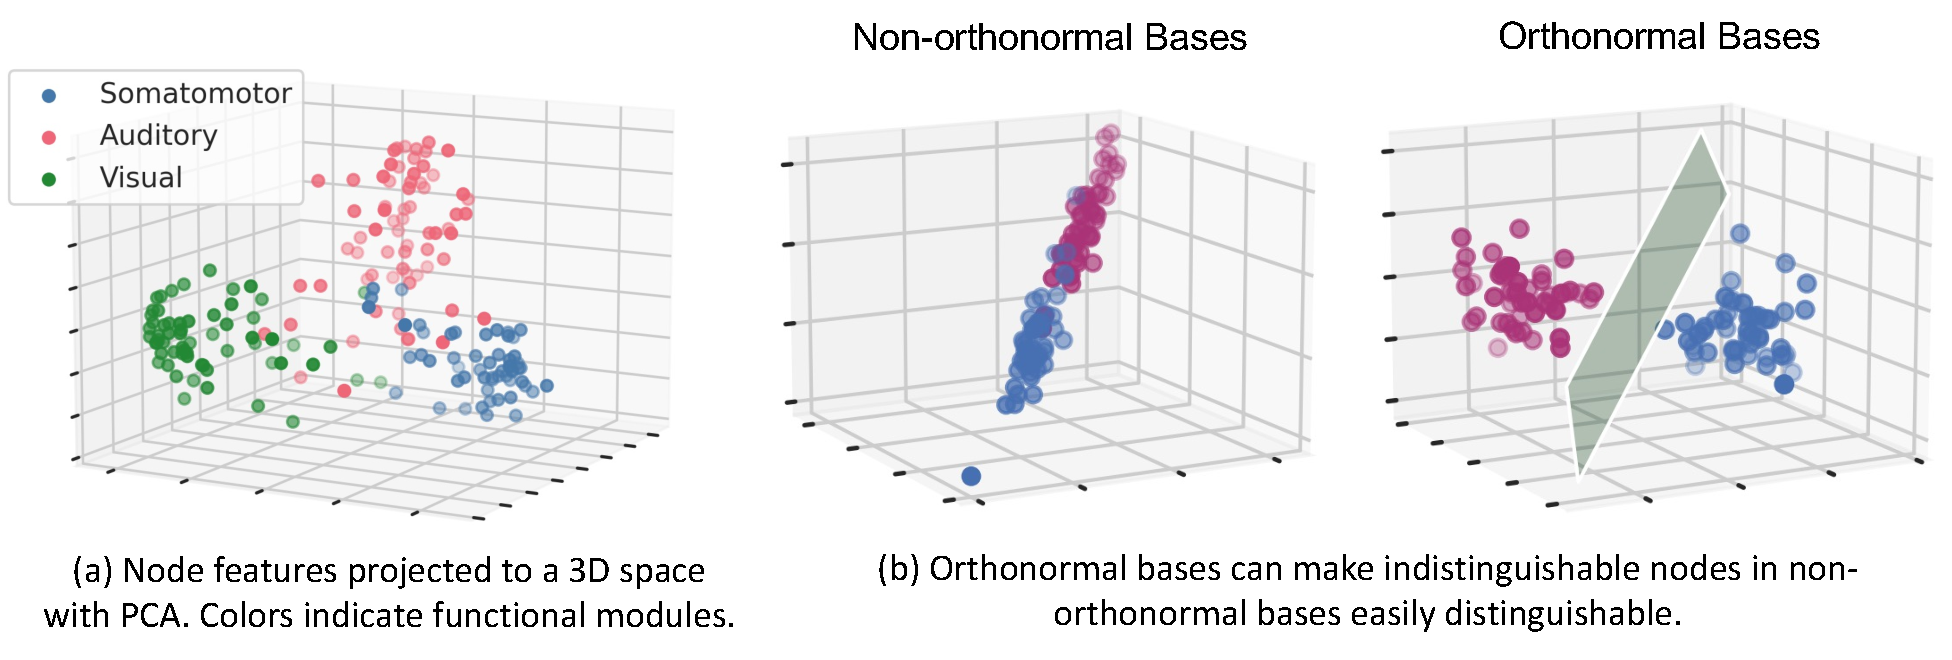
\includegraphics[width=0.9\columnwidth]{figure1} % Reduce the figure size so that it is slightly narrower than the column. Don't use precise values for figure width.This setup will avoid overfull boxes.
% \caption{Using the trim and clip commands produces fragile layers that can result in disasters (like this one from an actual paper) when the color space is corrected or the PDF combined with others for the final proceedings. Crop your figures properly in a graphics program -- not in LaTeX}.
% \label{fig1}
% \end{figure}

% \begin{figure*}[t]
% \centering
% \includegraphics[width=0.8\textwidth]{figure2} % Reduce the figure size so that it is slightly narrower than the column.
% \caption{Adjusting the bounding box instead of actually removing the unwanted data resulted multiple layers in this paper. It also needlessly increased the PDF size. In this case, the size of the unwanted layer doubled the paper's size, and produced the following surprising results in final production. Crop your figures properly in a graphics program. Don't just alter the bounding box.}
% \label{fig2}
% \end{figure*}

% % Using the \centering command instead of \begin{center} ... \end{center} will save space
% % Positioning your figure at the top of the page will save space and make the paper more readable
% % Using 0.95\columnwidth in conjunction with the


% Your paper must compile in PDF\LaTeX{}. Consequently, all your figures must be .jpg, .png, or .pdf. You may not use the .gif (the resolution is too low), .ps, or .eps file format for your figures.

% Figures, drawings, tables, and photographs should be placed throughout the paper on the page (or the subsequent page) where they are first discussed. Do not group them together at the end of the paper. If placed at the top of the paper, illustrations may run across both columns. Figures must not invade the top, bottom, or side margin areas. Figures must be inserted using the \textbackslash usepackage\{graphicx\}. Number figures sequentially, for example, figure 1, and so on. Do not use minipage to group figures.

% If you normally create your figures using pgfplots, please create the figures first, and then import them as pdfs with proper bounding boxes, as the bounding and trim boxes created by pfgplots are fragile and not valid.

% When you include your figures, you must crop them \textbf{outside} of \LaTeX{}. The command \textbackslash includegraphics*[clip=true, viewport 0 0 10 10]{...} might result in a PDF that looks great, but the image is \textbf{not really cropped.} The full image can reappear (and obscure whatever it is overlapping) when page numbers are applied or color space is standardized. Figures \ref{fig1}, and \ref{fig2} display some unwanted results that often occur.

% If your paper includes illustrations that are not compatible with PDF\TeX{} (such as .eps or .ps documents), you will need to convert them. The epstopdf package will usually work for eps files. You will need to convert your ps files to PDF however.

% \subsubsection {Figure Captions.}The illustration number and caption must appear \textit{under} the illustration. Labels, and other text with the actual illustration must be at least nine-point type. However, the font and size of figure captions must be 10 point roman. Do not make them smaller, bold, or italic. (Individual words may be italicized if the context requires differentiation.)

% \subsection{Tables}

% Tables should be presented in 10 point roman type. If necessary, they may be altered to 9 point type. You may not use any commands that further reduce point size below nine points. Tables that do not fit in a single column must be placed across double columns. If your table won't fit within the margins even when spanning both columns, you must split it. Do not use minipage to group tables.

% \subsubsection {Table Captions.} The number and caption for your table must appear \textit{under} (not above) the table.  Additionally, the font and size of table captions must be 10 point roman and must be placed beneath the figure. Do not make them smaller, bold, or italic. (Individual words may be italicized if the context requires differentiation.)



% \subsubsection{Low-Resolution Bitmaps.}
% You may not use low-resolution (such as 72 dpi) screen-dumps and GIF files---these files contain so few pixels that they are always blurry, and illegible when printed. If they are color, they will become an indecipherable mess when converted to black and white. This is always the case with gif files, which should never be used. The resolution of screen dumps can be increased by reducing the print size of the original file while retaining the same number of pixels. You can also enlarge files by manipulating them in software such as PhotoShop. Your figures should be 300 dpi when incorporated into your document.

% \subsubsection{\LaTeX{} Overflow.}
% \LaTeX{} users please beware: \LaTeX{} will sometimes put portions of the figure or table or an equation in the margin. If this happens, you need to make the figure or table span both columns. If absolutely necessary, you may reduce the figure, or reformat the equation, or reconfigure the table.{ \bf Check your log file!} You must fix any overflow into the margin (that means no overfull boxes in \LaTeX{}). \textbf{Nothing is permitted to intrude into the margin or gutter.}


% \subsubsection{Using Color.}
% Use of color is restricted to figures only. It must be WACG 2.0 compliant. (That is, the contrast ratio must be greater than 4.5:1 no matter the font size.) It must be CMYK, NOT RGB. It may never be used for any portion of the text of your paper. The archival version of your paper will be printed in black and white and grayscale. The web version must be readable by persons with disabilities. Consequently, because conversion to grayscale can cause undesirable effects (red changes to black, yellow can disappear, and so forth), we strongly suggest you avoid placing color figures in your document. If you do include color figures, you must (1) use the CMYK (not RGB) colorspace and (2) be mindful of readers who may happen to have trouble distinguishing colors. Your paper must be decipherable without using color for distinction.

% \subsubsection{Drawings.}
% We suggest you use computer drawing software (such as Adobe Illustrator or, (if unavoidable), the drawing tools in Microsoft Word) to create your illustrations. Do not use Microsoft Publisher. These illustrations will look best if all line widths are uniform (half- to two-point in size), and you do not create labels over shaded areas. Shading should be 133 lines per inch if possible. Use Times Roman or Helvetica for all figure call-outs. \textbf{Do not use hairline width lines} --- be sure that the stroke width of all lines is at least .5 pt. Zero point lines will print on a laser printer, but will completely disappear on the high-resolution devices used by our printers.

% \subsubsection{Photographs and Images.}
% Photographs and other images should be in grayscale (color photographs will not reproduce well; for example, red tones will reproduce as black, yellow may turn to white, and so forth) and set to a minimum of 300 dpi. Do not prescreen images.

% \subsubsection{Resizing Graphics.}
% Resize your graphics \textbf{before} you include them with LaTeX. You may \textbf{not} use trim or clip options as part of your \textbackslash includegraphics command. Resize the media box of your PDF using a graphics program instead.

% \subsubsection{Fonts in Your Illustrations.}
% You must embed all fonts in your graphics before including them in your LaTeX document.

% \subsection{References}
% The AAAI style includes a set of definitions for use in formatting references with BibTeX. These definitions make the bibliography style fairly close to the one specified below. To use these definitions, you also need the BibTeX style file ``aaai21.bst," available in the AAAI Author Kit on the AAAI web site. Then, at the end of your paper but before \textbackslash end{document}, you need to put the following lines:

% \begin{quote}
% \begin{small}
% \textbackslash bibliography\{bibfile1,bibfile2,...\}
% \end{small}
% \end{quote}

% Please note that the aaai21.sty class already sets the bibliographystyle for you, so you do not have to place any \textbackslash bibliographystyle command in the document yourselves. The aaai21.sty file is incompatible with the hyperref and navigator packages. If you use either, your references will be garbled and your paper will be returned to you.

% References may be the same size as surrounding text. However, in this section (only), you may reduce the size to \textbackslash small if your paper exceeds the allowable number of pages. Making it any smaller than 9 point with 10 point linespacing, however, is not allowed. A more precise and exact method of reducing the size of your references minimally is by means of the following command: \begin{quote}
% \textbackslash fontsize\{9.8pt\}\{10.8pt\}
% \textbackslash selectfont\end{quote}

% \noindent You must reduce the size equally for both font size and line spacing, and may not reduce the size beyond \{9.0pt\}\{10.0pt\}.

% The list of files in the \textbackslash bibliography command should be the names of your BibTeX source files (that is, the .bib files referenced in your paper).

% The following commands are available for your use in citing references:
% \begin{quote}
% {\em \textbackslash cite:} Cites the given reference(s) with a full citation. This appears as ``(Author Year)'' for one reference, or ``(Author Year; Author Year)'' for multiple references.\smallskip\\
% {\em \textbackslash shortcite:} Cites the given reference(s) with just the year. This appears as ``(Year)'' for one reference, or ``(Year; Year)'' for multiple references.\smallskip\\
% {\em \textbackslash citeauthor:} Cites the given reference(s) with just the author name(s) and no parentheses.\smallskip\\
% {\em \textbackslash citeyear:} Cites the given reference(s) with just the date(s) and no parentheses.
% \end{quote}



% Formatted bibliographies should look like the following examples.

% \smallskip \noindent \textit{Book with Multiple Authors}\\
% Engelmore, R., and Morgan, A. eds. 1986. \textit{Blackboard Systems.} Reading, Mass.: Addison-Wesley.

% \smallskip \noindent \textit{Journal Article}\\
% Robinson, A. L. 1980a. New Ways to Make Microcircuits Smaller. \textit{Science} 208: 1019--1026.

% \smallskip \noindent \textit{Magazine Article}\\
% Hasling, D. W.; Clancey, W. J.; and Rennels, G. R. 1983. Strategic Explanations in Consultation. \textit{The International Journal of Man-Machine Studies} 20(1): 3--19.

% \smallskip \noindent \textit{Proceedings Paper Published by a Society}\\
% Clancey, W. J. 1983. Communication, Simulation, and Intelligent Agents: Implications of Personal Intelligent Machines for Medical Education. In \textit{Proceedings of the Eighth International Joint Conference on Artificial Intelligence,} 556--560. Menlo Park, Calif.: International Joint Conferences on Artificial Intelligence, Inc.

% \smallskip \noindent \textit{Proceedings Paper Published by a Press or Publisher}\\
% Clancey, W. J. 1984. Classification Problem Solving. In \textit{Proceedings of the Fourth National Conference on Artificial Intelligence,} 49--54. Menlo Park, Calif.: AAAI Press.

% \smallskip \noindent \textit{University Technical Report}\\
% Rice, J. 1986. Poligon: A System for Parallel Problem Solving, Technical Report, KSL-86-19, Dept. of Computer Science, Stanford Univ.

% \smallskip \noindent \textit{Dissertation or Thesis}\\
% Clancey, W. J. 1979. Transfer of Rule-Based Expertise through a Tutorial Dialogue. Ph.D. diss., Dept. of Computer Science, Stanford Univ., Stanford, Calif.

% \smallskip \noindent \textit{Forthcoming Publication}\\
% Clancey, W. J. 2021. The Engineering of Qualitative Models. Forthcoming.

% For the most up to date version of the AAAI reference style, please consult the \textit{AI Magazine} Author Guidelines at \url{https://aaai.org/ojs/index.php/aimagazine/about/submissions#authorGuidelines}



% \section{Proofreading Your PDF}
% Please check all the pages of your PDF file. The most commonly forgotten element is the acknowledgements --- especially the correct grant number. Authors also commonly forget to add the metadata to the source, use the wrong reference style file, or don't follow the capitalization rules or comma placement for their author-title information properly. A final common problem is text (expecially equations) that runs into the margin. You will need to fix these common errors before submitting your file.

% \section{Improperly Formatted Files }
% In the past, AAAI has corrected improperly formatted files submitted by the authors. Unfortunately, this has become an increasingly burdensome expense that we can no longer absorb). Consequently, if your file is improperly formatted, it will be returned to you for correction.

% \subsection{\LaTeX{} 209 Warning}
% If you use \LaTeX{} 209 your paper will be returned to you unpublished. Convert your paper to \LaTeX{}2e.

% \section{Naming Your Electronic File}
% We require that you name your \LaTeX{} source file with the last name (family name) of the first author so that it can easily be differentiated from other submissions. Complete file-naming instructions will be provided to you in the submission instructions.

% \section{Submitting Your Electronic Files to AAAI}
% Instructions on paper submittal will be provided to you in your acceptance letter.

% \section{Inquiries}
% If you have any questions about the preparation or submission of your paper as instructed in this document, please contact AAAI Press at the address given below. If you have technical questions about implementation of the aaai style file, please contact an expert at your site. We do not provide technical support for \LaTeX{} or any other software package. To avoid problems, please keep your paper simple, and do not incorporate complicated macros and style files.

% \begin{quote}
% \noindent AAAI Press\\
% 2275 East Bayshore Road, Suite 160\\
% Palo Alto, California 94303\\
% \textit{Telephone:} (650) 328-3123\\
% \textit{E-mail:} See the submission instructions for your particular conference or event.
% \end{quote}

% \section{Additional Resources}
% \LaTeX{} is a difficult program to master. If you've used that software, and this document didn't help or some items were not explained clearly, we recommend you read Michael Shell's excellent document (testflow doc.txt V1.0a 2002/08/13) about obtaining correct PS/PDF output on \LaTeX{} systems. (It was written for another purpose, but it has general application as well). It is available at www.ctan.org in the tex-archive.

% \section{ Acknowledgments}
% AAAI is especially grateful to Peter Patel Schneider for his work in implementing the original aaai.sty file, liberally using the ideas of other style hackers, including Barbara Beeton. We also acknowledge with thanks the work of George Ferguson for his guide to using the style and BibTeX files --- which has been incorporated into this document --- and Hans Guesgen, who provided several timely modifications, as well as the many others who have, from time to time, sent in suggestions on improvements to the AAAI style. We are especially grateful to Francisco Cruz, Marc Pujol-Gonzalez, and Mico Loretan for the improvements to the Bib\TeX{} and \LaTeX{} files made in 2020.

% The preparation of the \LaTeX{} and Bib\TeX{} files that implement these instructions was supported by Schlumberger Palo Alto Research, AT\&T Bell Laboratories, Morgan Kaufmann Publishers, The Live Oak Press, LLC, and AAAI Press. Bibliography style changes were added by Sunil Issar. \verb+\+pubnote was added by J. Scott Penberthy. George Ferguson added support for printing the AAAI copyright slug. Additional changes to aaai21.sty and aaai21.bst have been made by Francisco Cruz, Marc Pujol-Gonzalez, and Mico Loretan.

% \bigskip
% \noindent Thank you for reading these instructions carefully. We look forward to receiving your electronic files!

\end{document}